\documentclass[a4paper]{scrartcl}

\usepackage[
fancytheorems,
fancyproofs,
noindent,
]{adam}

\usepackage{tikz}
\usepackage{bm}

\definecolor{mblue}{HTML}{1F5FA9}
\definecolor{mred}{HTML}{C0392B}
\definecolor{mgreen}{HTML}{1B7A4B}
\definecolor{morange}{HTML}{D98218}
\definecolor{mpurple}{HTML}{7B3FA0}

\tikzset{circ/.style={circle, fill, inner sep=1.15pt}}
\tikzset{ocirc/.style={circle, draw, fill=white, inner sep=1.05pt, line width=0.5pt}}

\newcommand{\ket}[1]{\left| #1 \right\rangle}
\newcommand{\bra}[1]{\left\langle #1 \right|}
\newcommand{\avg}[1]{\left\langle #1 \right\rangle}
\newcommand{\dbar}{\mathchar'26\mkern-11mu \mathrm{d}}

\title{Statistical Physics}
\author{Adam Kelly (\texttt{ak2316@cam.ac.uk})}
\date{\today}

\allowdisplaybreaks

\begin{document}

\maketitle

Every physics course we have met so far has been microscopic. We wrote down the equation of motion for a particle, or the Schr\"odinger equation for an electron in a hydrogen atom, and then we worked hard to solve it. Statistical physics asks what happens when we try to do this for $10^{23}$ particles at once. The honest answer is that we cannot: no computer will ever integrate Avogadro's number of coupled differential equations, and even if one could, the output would be useless to us. What saves the subject -- and makes it one of the most powerful in physics -- is that we do not \emph{want} to know what all $10^{23}$ particles are doing. We want to know a handful of macroscopic numbers: the pressure of the gas, its temperature, its heat capacity. The remarkable fact is that these few numbers can be extracted from the microscopic laws by an argument that is essentially probabilistic, and that the extraction is not merely approximate but, for systems this large, absurdly accurate.

The course has three faces. First we build the machinery: microstates, ensembles, entropy, temperature and the partition function, which is the single most useful object in the subject. Then we turn the machinery on real systems -- classical gases, and then quantum ones, where we will find that the same formalism produces blackbody radiation, the heat capacity of solids, the physics of white dwarf stars and the strange collective behaviour of Bose--Einstein condensates. Along the way we will meet \emph{classical thermodynamics}, which is the historical route into the subject: a set of laws about heat and work discovered before anyone was sure that atoms existed, and which we can now watch emerge from the statistics. Finally, we look at phase transitions, where a system changes its character discontinuously as we turn a knob, and where -- most surprisingly of all -- wildly different systems turn out to behave in exactly the same way.

This article constitutes my notes for the `Statistical Physics' course, held in Lent 2021 at Cambridge. These notes are \emph{not a transcription of the lectures}, and differ significantly in quite a few areas. Still, all lectured material should be covered\footnote{The course assumes a working knowledge of quantum mechanics at the level of the Part IB course, and it will help enormously to have met the Legendre transform, for instance in the Variational Principles course; I will remind the reader of what is needed as we go.}.

\tableofcontents

\section{Fundamentals of Statistical Mechanics}

We begin by setting up the framework of the subject. The ideas here are not difficult, but they are subtle, and they are the foundation for everything that follows -- so it is worth going slowly.

\subsection{Microstates and the Microcanonical Ensemble}

Our object of study is a system of $N$ particles, where $N$ is a very large number. The canonical picture to have in mind is a box of gas, sealed off from the rest of the universe. We begin by describing the system in as much detail as possible.

\begin{definition}[Microstate]
	A \vocab{microstate} of a system is a complete specification of its state: in the quantum setting, an actual state $\ket{n}$ of the full $N$-particle system.
\end{definition}

A microstate is a hopeless thing to try to write down. But the whole point of statistical physics is that we do not need to: enormously many microstates are macroscopically indistinguishable from one another, and we may as well treat them all on the same footing. So we adopt a probabilistic description. Let $\{\ket n\}$ be an orthonormal basis of energy eigenstates,
$$
\hat H \ket{n} = E_n \ket{n},
$$
and let $p(n)$ be the probability that our system is in the microstate $\ket n$. It is important to be clear about what kind of probability this is. It is \emph{not} a quantum amplitude squared; it is a classical probability, encoding our ignorance about which state the system is actually in. (If you have met density matrices, we are describing the mixed state $\rho = \sum_n p(n) \ket n \bra n$.)

\begin{definition}[Ensemble average]
	Given probabilities $p(n)$, the \vocab{expectation value} of an operator $\mathcal O$ is
	$$
	\avg{\mathcal O} = \sum_n p(n) \bra n \mathcal O \ket n.
	$$
\end{definition}

An equivalent and often more intuitive way to think about this: imagine $W \gg 1$ independent copies of our system, with $W p(n)$ of them in the microstate $\ket n$. This collection is called an \vocab{ensemble}, and $\avg{\mathcal O}$ is just the average of $\mathcal O$ over the ensemble. Which picture one uses makes no difference to the mathematics.

Throughout, we will assume our systems are in \vocab{equilibrium}, meaning that the distribution $p(n)$ does not change with time. This does not mean nothing is happening -- the molecules of a gas in equilibrium are hurtling about as fast as ever. It means only that the statistics are stationary. Systems out of equilibrium are enormously harder, and we will not touch them.

Now, what should $p(n)$ be? Suppose all we know about the system is its energy. The microstates consistent with what we know are called \vocab{accessible}, and the entire subject rests on the following assumption.

\begin{axiom}[Fundamental Assumption of Statistical Mechanics]
	An isolated system in equilibrium is equally likely to be found in any of its accessible microstates.
\end{axiom}

This is not something we can prove from the microscopic laws (proving it, in the guise of the \emph{ergodic hypothesis}, is genuinely hard and still not fully understood). We take it as an axiom and judge it by its consequences, which are spectacularly successful.

\begin{definition}[Microcanonical ensemble]
	In the \vocab{microcanonical ensemble} we take our partial knowledge to be that the energy lies in a window $[E, E + \delta E]$, where $\delta E$ is the resolution of our measuring apparatus. We write $\Omega(E)$ for the number of microstates with $E \leq E_n \leq E + \delta E$.
\end{definition}

The fundamental assumption then reads
$$
p(n) = \begin{cases}
	1/\Omega(E) & E \leq E_n \leq E + \delta E,\\
	0 & \text{otherwise.}
\end{cases}
$$
It looks worrying that the theory should depend on the arbitrary parameter $\delta E$, and we will see shortly that in fact it does not. Note also that it is essential here that we are working quantum mechanically: energy levels are discrete, so `counting states' makes sense. Doing this classically requires more care, and we will come back to it in Section~\ref{sec:classicalZ}.

\begin{example}
	Take $N = 10^{23}$ particles fixed in place, each of which can be in one of two states $\ket\uparrow, \ket\downarrow$ of the same energy $\varepsilon$. Then every configuration has total energy $N \varepsilon$, and
	$$
	\Omega(N\varepsilon) = 2^{10^{23}}.
	$$
	This is a completely preposterous number -- vastly larger than the number of atoms in the observable universe -- and it is entirely typical of the numbers in this subject.
\end{example}

Numbers like $2^{10^{23}}$ are unpleasant to work with, and worse, $\Omega$ is multiplicative rather than additive when we combine systems. Both problems are cured at a stroke by taking a logarithm.

\begin{definition}[Boltzmann entropy]
	The \vocab{entropy} of a system is
	$$
	S(E) = k \log \Omega(E),
	$$
	where $k = 1.381 \times 10^{-23}\,\mathrm{J}\,\mathrm{K}^{-1}$ is \vocab{Boltzmann's constant}.
\end{definition}

The constant $k$ is a historical accident: thermodynamics was developed before anyone knew about microstates, and temperature was given its own unit. Had physics been done in the other order we would simply have set $k = 1$ and measured temperature in joules.

We can now dispose of the worry about $\delta E$. If we double the width of our energy window we roughly double $\Omega$, and so we change $S$ by $k \log 2 \approx 10^{-23}\,\mathrm{J}\,\mathrm{K}^{-1}$. Meanwhile $S$ itself is of order $Nk \sim 1\,\mathrm{J}\,\mathrm{K}^{-1}$. So the dependence on $\delta E$ is utterly negligible, and we suppress it. This is the first instance of a pattern that recurs constantly: because $N$ is so large, factors that would be significant anywhere else in physics are invisible here.

The second virtue of the logarithm is additivity. If we have two \emph{non-interacting} systems with energies $E_1$ and $E_2$, then a microstate of the pair is a microstate of each, so $\Omega(E_1, E_2) = \Omega_1(E_1)\Omega_2(E_2)$ and hence
$$
S(E_1, E_2) = S_1(E_1) + S_2(E_2).
$$

\subsection{Entropy and the Second Law}

Additivity is not very interesting until we let the systems talk to each other. So suppose we now bring our two systems into contact and allow them to exchange energy, while keeping the total energy $E_{\mathrm{tot}} = E_1 + E_2$ fixed. Now the individual energies can fluctuate, and the number of states available to the combined system is
$$
\Omega(E_{\mathrm{tot}}) = \sum_{E_i} \Omega_1(E_i)\, \Omega_2(E_{\mathrm{tot}} - E_i) = \sum_{E_i} \exp\left( \frac{S_1(E_i) + S_2(E_{\mathrm{tot}} - E_i)}{k}\right),
$$
where the sum runs over the energy bins of width $\delta E$ that we chose earlier.

Now look at the size of the exponents. Each $S/k$ is of order $N \sim 10^{23}$. So if the exponent is even slightly larger for one term than for another, that term dominates the sum by a factor which is the exponential of something like $10^{20}$. In other words: \emph{the sum is completely dominated by its largest term.} Writing $E_*$ for the value of $E_i$ that maximises $S_1(E_i) + S_2(E_{\mathrm{tot}} - E_i)$, we have
$$
S(E_{\mathrm{tot}}) = k\log \Omega(E_{\mathrm{tot}}) \approx S_1(E_*) + S_2(E_{\mathrm{tot}} - E_*).
$$
Of course some neighbouring terms also contribute, but including them multiplies $\Omega$ by some modest factor and hence adds something of order $k$ to $S$, which we cheerfully ignore.

The same estimate tells us something much stronger. The probability that the first system has energy $E_1$ (writing $E_2 = E_{\mathrm{tot}} - E_1$) is
$$
\frac{\Omega_1(E_1)\Omega_2(E_2)}{\Omega(E_{\mathrm{tot}})} = \exp\left( \frac{S_1(E_1) + S_2(E_2) - S(E_{\mathrm{tot}})}{k} \right).
$$
Unless $S_1(E_1) + S_2(E_2)$ agrees with its maximum value to fantastic precision, this probability is effectively zero. So although $E_1$ is in principle free to fluctuate, in practice it is pinned to $E_*$ to a precision far beyond anything we could measure.

Finally, suppose we prepare the two systems separately with $E_1 \neq E_*$ and only then bring them together. The system is not in equilibrium; it will evolve, $E_1$ will drift to $E_*$, and in doing so the entropy will increase from $S_1(E_1) + S_2(E_2)$ to its maximum value. This is the second law.

\begin{law}[Second Law of Thermodynamics]
	The entropy of an isolated system never decreases, and in equilibrium it attains its maximum value.
\end{law}

It is worth being precise about what we have and have not shown. We have not shown that entropy decrease is \emph{impossible}. What we have shown is that it is overwhelmingly improbable -- the odds against it are the exponential of $10^{23}$. This is a much more satisfying state of affairs than a bald prohibition, because it explains why the second law has the peculiar status it does: it is a law of statistics rather than of mechanics, and it is the only law of physics that distinguishes the future from the past.

\subsection{Temperature}

We have a function $S(E)$. The obvious thing to do with it is differentiate it, and the obvious thing to do with the answer is give it a name.

\begin{definition}[Temperature]
	The \vocab{temperature} of a system is defined by
	$$
	\frac{1}{T} = \frac{\dd S}{\dd E}.
	$$
\end{definition}

Why should this deserve to be called temperature? Because it does what temperature is supposed to do. Let us check the two most basic properties we expect.

\begin{proposition}
	Two systems in thermal contact and in equilibrium have the same temperature.
\end{proposition}
\begin{proof}
	We found the equilibrium energy $E_*$ by maximising $S_1(E_1) + S_2(E_{\mathrm{tot}} - E_1)$ over $E_1$. Differentiating and setting the result to zero,
	$$
	\left.\frac{\dd S_1}{\dd E}\right|_{E_1 = E_*} = \left.\frac{\dd S_2}{\dd E}\right|_{E_2 = E_{\mathrm{tot}} - E_*},
	$$
	that is, $1/T_1 = 1/T_2$, so $T_1 = T_2$.
\end{proof}

\begin{proposition}
	If two systems at temperatures $T_1 > T_2$ are brought into contact, energy flows from the first to the second.
\end{proposition}
\begin{proof}
	The systems are not in equilibrium, so some energy is transferred. Say after a short time $E_1 \mapsto E_1 + \delta E$ and $E_2 \mapsto E_2 - \delta E$. The change in total entropy is
	$$
	\delta S = \frac{\dd S_1}{\dd E}\delta E - \frac{\dd S_2}{\dd E}\delta E = \left(\frac{1}{T_1} - \frac{1}{T_2}\right)\delta E.
	$$
	By hypothesis $1/T_1 - 1/T_2 < 0$, and by the second law $\delta S > 0$. Hence $\delta E < 0$: the first system loses energy.
\end{proof}

So heat flows from hot to cold, and bodies in equilibrium have equal temperatures. Notice that these arguments used nothing about $T$ except that $1/T$ is a decreasing function of $T$; we could have defined $\dd S/\dd E$ to be any monotone decreasing function of `temperature' and got the same results. What singles out this particular choice is that it agrees with the temperature scale everyone already used -- the one defined by the ideal gas law -- as we will verify in Section~\ref{sec:idealgas}.

\subsection{Heat Capacity, and a First Example}

Differentiating $S$ gave us temperature. If we now invert $T = T(E)$ to get $E = E(T)$ and differentiate again, we get another familiar quantity.

\begin{definition}[Heat capacity]
	The \vocab{heat capacity} of a system is
	$$
	C = \frac{\dd E}{\dd T}.
	$$
	The \vocab{specific heat capacity} is $C$ divided by the mass of the system.
\end{definition}

Unlike $\Omega$ or $S$, this is something we can go into a laboratory and measure: pump in a known amount of energy, and see how much the temperature rises. And measuring it gives us the entropy for free, because
$$
\frac{\dd S}{\dd T} = \frac{\dd S}{\dd E}\frac{\dd E}{\dd T} = \frac{C}{T},
$$
and hence, integrating,
$$
\Delta S = \int_{T_1}^{T_2} \frac{C(T)}{T} \dd T.
$$
So although entropy was defined by counting microstates -- a thoroughly theoretical operation -- its changes are experimentally accessible.

The heat capacity also settles a loose end. When we found $E_*$ by setting a derivative to zero, we only checked that it was a stationary point. Differentiating once more,
$$
\frac{\dd^2 S}{\dd E^2} = \frac{\dd}{\dd E}\left(\frac 1T\right) = -\frac{1}{T^2}\frac{\dd T}{\dd E} = -\frac{1}{T^2 C},
$$
so $S_1 + S_2$ has a genuine maximum at $E_*$ provided $C_1, C_2 > 0$. Positivity of heat capacity is thus exactly the condition for thermal equilibrium to be stable.

Enough generalities. Let us compute something.

\begin{example}[The two-state system]
	Take $N$ non-interacting particles fixed at lattice sites, each of which has two states, with energies
	$$
	E_\downarrow = 0, \qquad E_\uparrow = \varepsilon.
	$$
	Think of these as spins in a magnetic field. If $N_\uparrow$ of them are excited then the total energy is $E = \varepsilon N_\uparrow$, and (choosing $\delta E < \varepsilon$, which is legitimate here) the number of microstates is just the number of ways of choosing which particles are excited:
	$$
	\Omega(E) = \binom{N}{N_\uparrow} = \frac{N!}{N_\uparrow!\,(N - N_\uparrow)!}.
	$$
	To make progress we need \vocab{Stirling's approximation}, which we will use constantly:
	$$
	\log N! = N\log N - N + \tfrac 12 \log(2\pi N) + O(1/N).
	$$
	Since $N \sim 10^{23}$ we keep only the first two terms. Applying this three times and writing $x = E/(N\varepsilon) = N_\uparrow/N$ for the fraction of excited particles,
	\begin{align*}
		S(E) &= k\big(N\log N - N_\uparrow \log N_\uparrow - (N - N_\uparrow)\log(N - N_\uparrow)\big)\\
		&= -kN\Big( x \log x + (1-x)\log(1-x)\Big).
	\end{align*}
	This is much more illuminating when plotted.
	\begin{center}
		\begin{tikzpicture}
			\draw [->] (0,0) -- (6.9,0) node [right] {$E$};
			\draw [->] (0,0) -- (0,3.9) node [above] {$S(E)$};
			\draw [thick, mblue] plot coordinates {(0.001,0.005) (0.068,0.286) (0.135,0.498) (0.203,0.682) (0.270,0.848) (0.338,1.000) (0.405,1.141) (0.472,1.273) (0.540,1.396) (0.607,1.513) (0.675,1.623) (0.742,1.727) (0.809,1.826) (0.877,1.920) (0.944,2.010) (1.012,2.094) (1.079,2.175) (1.146,2.252) (1.214,2.325) (1.281,2.394) (1.349,2.460) (1.416,2.523) (1.483,2.582) (1.551,2.638) (1.618,2.691) (1.686,2.742) (1.753,2.789) (1.820,2.833) (1.888,2.875) (1.955,2.914) (2.023,2.950) (2.090,2.984) (2.157,3.015) (2.225,3.044) (2.292,3.070) (2.360,3.094) (2.427,3.115) (2.494,3.134) (2.562,3.151) (2.629,3.165) (2.697,3.176) (2.764,3.186) (2.831,3.193) (2.899,3.197) (2.966,3.200) (3.034,3.200) (3.101,3.197) (3.169,3.193) (3.236,3.186) (3.303,3.176) (3.371,3.165) (3.438,3.151) (3.506,3.134) (3.573,3.115) (3.640,3.094) (3.708,3.070) (3.775,3.044) (3.843,3.015) (3.910,2.984) (3.977,2.950) (4.045,2.914) (4.112,2.875) (4.180,2.833) (4.247,2.789) (4.314,2.742) (4.382,2.691) (4.449,2.638) (4.517,2.582) (4.584,2.523) (4.651,2.460) (4.719,2.394) (4.786,2.325) (4.854,2.252) (4.921,2.175) (4.988,2.094) (5.056,2.010) (5.123,1.920) (5.191,1.826) (5.258,1.727) (5.325,1.623) (5.393,1.513) (5.460,1.396) (5.528,1.273) (5.595,1.141) (5.662,1.000) (5.730,0.848) (5.797,0.682) (5.865,0.498) (5.932,0.286) (5.999,0.005)};
			\draw [dashed] (3,0) -- (3,3.200) -- (0,3.200) node [left] {$Nk\log 2$};
			\node [below] at (3,0) {$\tfrac 12 N\varepsilon$};
			\node [below] at (6,0) {$N\varepsilon$};
			\node [below left] at (0,0) {$0$};
		\end{tikzpicture}
	\end{center}
	The entropy vanishes at $E = 0$ (all spins down: one microstate) and at $E = N\varepsilon$ (all spins up: one microstate), and is maximal in between at $E = N\varepsilon/2$, where it takes the value $Nk\log 2$ -- exactly what we expect, since then each spin is free to do as it pleases.

	Now differentiate to get the temperature:
	$$
	\frac 1T = \frac{\dd S}{\dd E} = \frac k\varepsilon \log\left(\frac{N\varepsilon}{E} - 1\right),
	$$
	which we can invert to give the beautifully simple
	$$
	\frac{N_\uparrow}{N} = \frac{E}{N\varepsilon} = \frac{1}{e^{\varepsilon/kT} + 1}.
	$$
	As $T \to 0$ we get $N_\uparrow \to 0$: everything falls into the ground state, as it should. As $T \to \infty$ we get $N_\uparrow/N \to \tfrac 12$, which is more surprising -- one might have guessed that infinite temperature would push everything into the excited state. It does not: at infinite temperature the Boltzmann factors for the two levels become equal and the spins are simply randomised.

	This has a strange consequence. The graph of $S$ against $E$ has negative slope for $E > N\varepsilon/2$, so such states have \emph{negative temperature}. Moreover, to get from positive $T$ to negative $T$ one must pass through $T = \infty$, so negative temperatures are `hotter' than infinite temperature. This is not a pathology of the definition but a genuine feature of systems whose energy is bounded above; it can only happen because we have frozen the particles in place and thrown away their kinetic energy, which is unbounded. Negative-temperature states have been produced in the laboratory, using nuclear spins in a crystal: align them with a magnetic field, then suddenly reverse the field.

	Finally, the heat capacity. Differentiating $E = N\varepsilon/(e^{\varepsilon/kT}+1)$,
	$$
	C = \frac{\dd E}{\dd T} = \frac{N\varepsilon^2}{kT^2}\, \frac{e^{\varepsilon/kT}}{\left(e^{\varepsilon/kT}+1\right)^2},
	$$
	which looks like this.
	\begin{center}
		\begin{tikzpicture}
			\draw [->] (0,0) -- (7.3,0) node [right] {$T$};
			\draw [->] (0,0) -- (0,3.7) node [above] {$C$};
			\draw [thick, mblue] plot coordinates {(0.093,0.000) (0.163,0.001) (0.233,0.033) (0.303,0.194) (0.372,0.541) (0.442,1.026) (0.512,1.554) (0.582,2.048) (0.651,2.462) (0.721,2.778) (0.791,2.997) (0.861,3.129) (0.931,3.191) (1.000,3.196) (1.070,3.160) (1.140,3.092) (1.210,3.003) (1.279,2.900) (1.349,2.789) (1.419,2.673) (1.489,2.556) (1.558,2.440) (1.628,2.327) (1.698,2.217) (1.768,2.112) (1.837,2.011) (1.907,1.915) (1.977,1.825) (2.047,1.738) (2.116,1.657) (2.186,1.580) (2.256,1.508) (2.326,1.440) (2.396,1.375) (2.465,1.315) (2.535,1.257) (2.605,1.203) (2.675,1.153) (2.744,1.105) (2.814,1.059) (2.884,1.017) (2.954,0.976) (3.023,0.938) (3.093,0.902) (3.163,0.868) (3.233,0.835) (3.302,0.805) (3.372,0.775) (3.442,0.748) (3.512,0.721) (3.582,0.696) (3.651,0.673) (3.721,0.650) (3.791,0.629) (3.861,0.608) (3.930,0.589) (4.000,0.570) (4.070,0.552) (4.140,0.535) (4.209,0.519) (4.279,0.503) (4.349,0.488) (4.419,0.474) (4.488,0.460) (4.558,0.447) (4.628,0.435) (4.698,0.423) (4.768,0.411) (4.837,0.400) (4.907,0.389) (4.977,0.379) (5.047,0.369) (5.116,0.360) (5.186,0.351) (5.256,0.342) (5.326,0.333) (5.395,0.325) (5.465,0.317) (5.535,0.310) (5.605,0.302) (5.674,0.295) (5.744,0.288) (5.814,0.282) (5.884,0.275) (5.954,0.269) (6.023,0.263) (6.093,0.258) (6.163,0.252) (6.233,0.247) (6.302,0.241) (6.372,0.236) (6.442,0.231) (6.512,0.227) (6.581,0.222) (6.651,0.217) (6.721,0.213) (6.791,0.209) (6.860,0.205) (6.930,0.201) (7.000,0.197)};
			\draw [dashed] (0.972,0) -- (0.972,3.200);
			\node [below] at (0.972,0) {\small $kT \sim \varepsilon$};
			\node [below left] at (0,0) {$0$};
		\end{tikzpicture}
	\end{center}
	Three things are worth noticing. First, the position of the peak is set by the microscopic energy gap, $kT \sim \varepsilon$; so a macroscopic measurement of $C$ tells us about the microscopic level structure. Secondly, as $T \to 0$ we have $C \propto T^{-2}e^{-\varepsilon/kT}$, which vanishes faster than any power of $T$ -- the classic analysis example of a smooth non-analytic function. This exponential suppression is the signature of an energy gap: at low temperatures there is simply not enough thermal energy to excite anything. Thirdly, $C \to 0$ at high temperature as well, which is peculiar and again a consequence of the bounded energy spectrum; a realistic system has $C$ increasing with $T$. In a real solid this spin contribution is swamped by the phonons and electrons, and shows up only as a small bump at low temperature, called a \vocab{Schottky anomaly}.
\end{example}

\subsection{Pressure, Volume and the First Law}

So far our systems have had exactly one macroscopic parameter, the energy. Real systems have more. The most obvious is volume: if we let the walls of our box move, then the energy eigenvalues change, and so $\Omega$ and $S$ depend on $V$ as well:
$$
S(E,V) = k\log \Omega(E,V).
$$
We must therefore be careful about what is held fixed when we differentiate, and we adopt the standard notation of writing the fixed variables as a subscript.

\begin{definition}[Temperature and pressure]
	For a system with variable volume,
	$$
	\frac 1T = \left(\frac{\partial S}{\partial E}\right)_V, \qquad p = T\left(\frac{\partial S}{\partial V}\right)_E.
	$$
\end{definition}

The definition of $p$ looks unmotivated, but it is forced on us by the same argument as before.

\begin{proposition}
	If two systems can exchange both energy and volume, with $E_1 + E_2$ and $V_1 + V_2$ fixed, then entropy is maximised when $T_1 = T_2$ and $p_1 = p_2$.
\end{proposition}
\begin{proof}
	We must maximise $S_1(E_1, V_1) + S_2(E_{\mathrm{tot}} - E_1, V_{\mathrm{tot}} - V_1)$ over both $E_1$ and $V_1$. The $E$ derivative gives $T_1 = T_2$ as before, and the $V$ derivative gives
	$$
	\left(\frac{\partial S_1}{\partial V}\right)_E = \left(\frac{\partial S_2}{\partial V}\right)_E,
	$$
	which, on multiplying by the common temperature, is $p_1 = p_2$.
\end{proof}

So $p$ is the quantity that equalises when a piston between two gases is free to move -- which is exactly what mechanical pressure does. To see that it really \emph{is} force per unit area, write $S = S(E,V)$ and take the total differential:
$$
\dd S = \left(\frac{\partial S}{\partial E}\right)_V \dd E + \left(\frac{\partial S}{\partial V}\right)_E \dd V = \frac{1}{T}\dd E + \frac pT \dd V.
$$
Rearranging gives one of the most important equations in the subject.

\begin{proposition}[First Law of Thermodynamics]
	$$
	\dd E = T \dd S - p \dd V.
	$$
\end{proposition}

The interpretation is this: $-p\,\dd V$ is the mechanical work done on the system when we compress it, exactly as in Newtonian mechanics, which confirms that our $p$ is the ordinary pressure. The remaining term $T \dd S$ is therefore energy transferred \emph{not} as mechanical work; we call it \vocab{heat}. The first law says that energy is conserved provided we remember to count heat as a form of energy -- a statement that took most of the nineteenth century to become uncontroversial.

\begin{example}[The ideal gas, done the hard way]\label{ex:idealmicro}
	Let us extract the equation of state of an ideal gas from the microcanonical ensemble. We will do this much more slickly later, so treat this as a demonstration that it \emph{can} be done. For $N$ free particles in a box of volume $V$, the accessible phase space at fixed energy $E$ factorises into a position part and a momentum part. Each particle can be anywhere in the box, giving a factor $V^N$; and the momenta are constrained to the sphere $\sum_i \vv p_i^2 = 2mE$ in $3N$ dimensions, whose area depends only on $E$ and $N$. So
	$$
	\Omega(E,V) = V^N f(E)
	$$
	for some function $f$ we do not need to know. Then $S = Nk \log V + k \log f(E)$, and
	$$
	p = T\left(\frac{\partial S}{\partial V}\right)_E = \frac{NkT}{V},
	$$
	which is the ideal gas law $pV = NkT$. Notice how little we had to know: only that the positions and momenta decouple.
\end{example}

\subsection{The Canonical Ensemble}\label{sec:canonical}

The microcanonical ensemble is conceptually clean but computationally awful: to use it we must count states at fixed energy, which usually means a nasty combinatorial problem. Worse, it is not a realistic description of most experiments. A beaker of water on a bench is not isolated; it is in contact with the room, and its energy fluctuates. What is fixed is its \emph{temperature}. This suggests a different setup, and it turns out to be enormously easier to work with.

So: let our system $\mathcal S$ be in thermal contact with a \vocab{reservoir} $\mathcal R$, so much larger than $\mathcal S$ that its temperature $T$ is unaffected by anything $\mathcal S$ does. The combined system is isolated, with total energy $E_{\mathrm{tot}}$, and we apply the microcanonical ensemble to \emph{it}. If $\mathcal S$ is in a definite microstate $\ket n$ of energy $E_n$, then the number of microstates of the combination is just the number available to the reservoir, namely $\Omega_{\mathcal R}(E_{\mathrm{tot}} - E_n)$. Hence
$$
p(n) \propto \Omega_{\mathcal R}(E_{\mathrm{tot}} - E_n) = \exp\left(\frac{S_{\mathcal R}(E_{\mathrm{tot}} - E_n)}{k}\right).
$$
Now $E_n \ll E_{\mathrm{tot}}$, so we may Taylor expand:
$$
S_{\mathcal R}(E_{\mathrm{tot}} - E_n) = S_{\mathcal R}(E_{\mathrm{tot}}) - E_n \left.\frac{\partial S_{\mathcal R}}{\partial E}\right|_{E_{\mathrm{tot}}} + \cdots = S_{\mathcal R}(E_{\mathrm{tot}}) - \frac{E_n}{T} + \cdots,
$$
and the higher terms are suppressed by further powers of $E_n/E_{\mathrm{tot}}$. The first term is a constant, independent of $n$, so it is absorbed into the normalisation, and we are left with the single most important formula of the course.

\begin{definition}[Boltzmann distribution and partition function]
	A system in equilibrium with a reservoir at temperature $T$ occupies its microstates with probabilities
	$$
	p(n) = \frac{e^{-\beta E_n}}{Z}, \qquad \beta = \frac{1}{kT},
	$$
	where the normalising constant
	$$
	Z = \sum_n e^{-\beta E_n}
	$$
	is the \vocab{partition function}. This probability distribution is the \vocab{Boltzmann distribution}, and the ensemble is the \vocab{canonical ensemble}.
\end{definition}

The sum defining $Z$ runs over all \emph{states}, not all energy levels; a level of degeneracy $g$ contributes $g e^{-\beta E}$. The factor $e^{-\beta E_n}$ is called the \vocab{Boltzmann factor}, and its shape is the whole story of the canonical ensemble: high-energy states are exponentially rare, and the scale on which `high' is measured is $kT$.

\begin{center}
	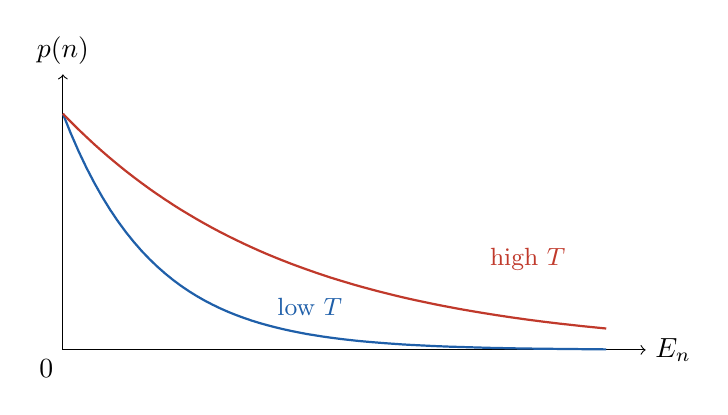
\begin{tikzpicture}
		\draw [->] (0,0) -- (7.4,0) node [right] {$E_n$};
		\draw [->] (0,0) -- (0,3.5) node [above] {$p(n)$};
		\draw [thick, mblue] plot coordinates {(0.000,3.000) (0.100,2.750) (0.200,2.521) (0.300,2.311) (0.400,2.119) (0.500,1.942) (0.600,1.780) (0.700,1.632) (0.800,1.496) (0.900,1.372) (1.000,1.257) (1.100,1.153) (1.200,1.057) (1.300,0.969) (1.400,0.888) (1.500,0.814) (1.600,0.746) (1.700,0.684) (1.800,0.627) (1.900,0.575) (2.000,0.527) (2.100,0.483) (2.200,0.443) (2.300,0.406) (2.400,0.372) (2.500,0.341) (2.600,0.313) (2.700,0.287) (2.800,0.263) (2.900,0.241) (3.000,0.221) (3.100,0.202) (3.200,0.186) (3.300,0.170) (3.400,0.156) (3.500,0.143) (3.600,0.131) (3.700,0.120) (3.800,0.110) (3.900,0.101) (4.000,0.093) (4.100,0.085) (4.200,0.078) (4.300,0.071) (4.400,0.065) (4.500,0.060) (4.600,0.055) (4.700,0.050) (4.800,0.046) (4.900,0.042) (5.000,0.039) (5.100,0.036) (5.200,0.033) (5.300,0.030) (5.400,0.027) (5.500,0.025) (5.600,0.023) (5.700,0.021) (5.800,0.019) (5.900,0.018) (6.000,0.016) (6.100,0.015) (6.200,0.014) (6.300,0.013) (6.400,0.011) (6.500,0.011) (6.600,0.010) (6.700,0.009) (6.800,0.008) (6.900,0.007)};
		\draw [thick, mred] plot coordinates {(0.000,3.000) (0.100,2.897) (0.200,2.798) (0.300,2.703) (0.400,2.610) (0.500,2.521) (0.600,2.435) (0.700,2.352) (0.800,2.271) (0.900,2.194) (1.000,2.119) (1.100,2.046) (1.200,1.976) (1.300,1.909) (1.400,1.843) (1.500,1.780) (1.600,1.720) (1.700,1.661) (1.800,1.604) (1.900,1.549) (2.000,1.496) (2.100,1.445) (2.200,1.396) (2.300,1.348) (2.400,1.302) (2.500,1.257) (2.600,1.214) (2.700,1.173) (2.800,1.133) (2.900,1.094) (3.000,1.057) (3.100,1.021) (3.200,0.986) (3.300,0.952) (3.400,0.919) (3.500,0.888) (3.600,0.858) (3.700,0.828) (3.800,0.800) (3.900,0.773) (4.000,0.746) (4.100,0.721) (4.200,0.696) (4.300,0.672) (4.400,0.649) (4.500,0.627) (4.600,0.606) (4.700,0.585) (4.800,0.565) (4.900,0.546) (5.000,0.527) (5.100,0.509) (5.200,0.492) (5.300,0.475) (5.400,0.459) (5.500,0.443) (5.600,0.428) (5.700,0.413) (5.800,0.399) (5.900,0.385) (6.000,0.372) (6.100,0.359) (6.200,0.347) (6.300,0.335) (6.400,0.324) (6.500,0.313) (6.600,0.302) (6.700,0.292) (6.800,0.282) (6.900,0.272)};
		\node [mblue, right] at (2.6,0.55) {\small low $T$};
		\node [mred, right] at (5.3,1.15) {\small high $T$};
		\node [below left] at (0,0) {$0$};
	\end{tikzpicture}
\end{center}

It is worth pausing over what this means for the occupation of energy levels. At low temperature almost all the probability sits in the ground state; as $T$ rises, states higher up the ladder become accessible, and the population spreads out. Schematically:

\begin{center}
	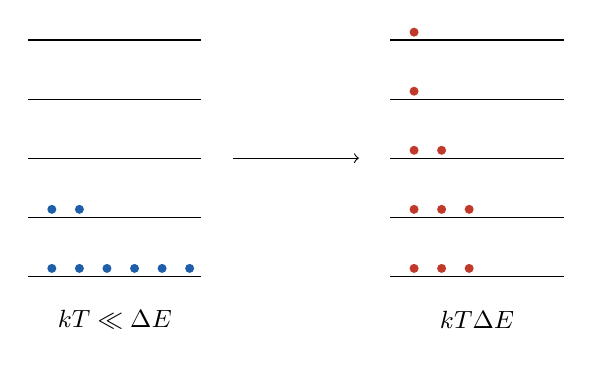
\begin{tikzpicture}[scale=1]
		% low T
		\begin{scope}
			\foreach \y in {0,0.75,1.5,2.25,3} {\draw [thin] (0,\y) -- (2.2,\y);}
			\foreach \x in {0.3,0.65,1,1.35,1.7,2.05} {\node [circ, mblue] at (\x,0.1) {};}
			\node [circ, mblue] at (0.3,0.85) {};
			\node [circ, mblue] at (0.65,0.85) {};
			\node at (1.1,-0.55) {\small $kT \ll \Delta E$};
		\end{scope}
		% high T
		\begin{scope}[xshift=4.6cm]
			\foreach \y in {0,0.75,1.5,2.25,3} {\draw [thin] (0,\y) -- (2.2,\y);}
			\node [circ, mred] at (0.3,0.1) {};
			\node [circ, mred] at (0.65,0.1) {};
			\node [circ, mred] at (1,0.1) {};
			\node [circ, mred] at (0.3,0.85) {};
			\node [circ, mred] at (0.65,0.85) {};
			\node [circ, mred] at (1,0.85) {};
			\node [circ, mred] at (0.3,1.6) {};
			\node [circ, mred] at (0.65,1.6) {};
			\node [circ, mred] at (0.3,2.35) {};
			\node [circ, mred] at (0.3,3.1) {};
			\node at (1.1,-0.55) {\small $kT \gtrsim \Delta E$};
		\end{scope}
		\draw [->] (2.6,1.5) -- (4.2,1.5);
	\end{tikzpicture}
\end{center}

The partition function was introduced as a normalisation constant, but it is far more useful than that: essentially every thermodynamic quantity can be got out of it by differentiation. The first example is the average energy.

\begin{proposition}
	The mean energy of a system in the canonical ensemble is
	$$
	\avg E = \sum_n p(n) E_n = -\frac{\partial}{\partial \beta}\log Z.
	$$
\end{proposition}
\begin{proof}
	Differentiating $Z = \sum_n e^{-\beta E_n}$ with respect to $\beta$ gives $\partial_\beta Z = -\sum_n E_n e^{-\beta E_n}$, and dividing by $Z$ gives $-\avg E$.
\end{proof}

Since $\avg E$ is what we actually mean by `the energy' of a macroscopic system, we will from now on drop the angle brackets and simply write $E$.

Before computing anything, one more structural remark, which is the reason the canonical ensemble is so much nicer than the microcanonical one. Suppose our system consists of two non-interacting parts, so that the states are pairs and the energies add. Then
$$
Z = \sum_{n_1, n_2} e^{-\beta (E_{n_1} + E_{n_2})} = \left(\sum_{n_1} e^{-\beta E_{n_1}}\right)\left(\sum_{n_2} e^{-\beta E_{n_2}}\right) = Z_1 Z_2.
$$
Partition functions of independent systems simply multiply. In the microcanonical ensemble the analogous statement was a convolution, which is why everything there was hard.

\begin{example}[The two-state system again]
	Each particle has $Z_1 = 1 + e^{-\beta \varepsilon}$, so for $N$ of them $Z = (1+e^{-\beta\varepsilon})^N$ and
	$$
	E = -\frac{\partial}{\partial\beta} \log Z = -N \frac{\partial}{\partial \beta}\log(1+e^{-\beta\varepsilon}) = \frac{N\varepsilon}{e^{\beta\varepsilon}+1},
	$$
	reproducing in three lines what took us a page of Stirling's formula in the microcanonical ensemble.
\end{example}

\subsection{Fluctuations}

There is an obvious objection to all this. In the microcanonical ensemble the energy was fixed; in the canonical ensemble it fluctuates. Why should the two give the same answers? The resolution is that the fluctuations are tiny, and we can quantify this precisely.

\begin{proposition}
	In the canonical ensemble,
	$$
	\Delta E^2 = \avg{E^2} - \avg E^2 = \frac{\partial^2}{\partial\beta^2}\log Z = k T^2 C_V.
	$$
\end{proposition}
\begin{proof}
	We compute
	$$
	\frac{\partial^2 \log Z}{\partial \beta^2} = \frac{\partial}{\partial\beta}\left(\frac{1}{Z}\frac{\partial Z}{\partial\beta}\right) = \frac{1}{Z}\frac{\partial^2 Z}{\partial \beta^2} - \left(\frac 1Z \frac{\partial Z}{\partial \beta}\right)^2 = \avg{E^2} - \avg E^2.
	$$
	On the other hand $\avg E = -\partial_\beta \log Z$, so this equals $-\partial \avg E/\partial\beta$; and since $\beta = 1/kT$ we have $\partial/\partial\beta = -kT^2\, \partial/\partial T$, giving $kT^2 (\partial E/\partial T)_V = kT^2 C_V$.
\end{proof}

Now, both $E$ and $C_V$ are proportional to $N$. So
$$
\frac{\Delta E}{E} \sim \frac{\sqrt N}{N} = \frac{1}{\sqrt N},
$$
which for $N \sim 10^{23}$ is about $10^{-12}$. The energy of a macroscopic system in the canonical ensemble is therefore fixed to about twelve significant figures, which is rather better than any experiment can do. This is why the two ensembles agree: in the thermodynamic limit the distinction between `fixed energy' and `fixed temperature' is invisible. We will use whichever is more convenient, which is almost always the canonical one.

The relation $\Delta E^2 = kT^2 C_V$ is also our first \vocab{fluctuation--dissipation relation}: it connects the size of spontaneous fluctuations (the left side) to the response of the system to an external prod (the right side). Relations of this type run through the whole of statistical physics.

\subsection{The Gibbs Entropy}

We defined entropy by counting microstates, which only makes sense when all accessible microstates are equally likely. In the canonical ensemble they are not, so we need a definition that works for a general probability distribution. Here it is.

\begin{definition}[Gibbs entropy]
	Given a probability distribution $p(n)$ over microstates, the \vocab{Gibbs entropy} is
	$$
	S = -k \sum_n p(n) \log p(n).
	$$
\end{definition}

This agrees with the old definition when it applies: if $p(n) = 1/\Omega$ on $\Omega$ accessible states, then
$$
S = -k\sum_{n} \frac{1}{\Omega}\log\frac 1\Omega = k\log\Omega
$$
as required. And it is exactly the quantity Shannon later introduced as a measure of the information content of a distribution -- entropy is a measure of how much we \emph{don't} know about the system, which is a rather satisfying way to think about the second law.

Let us check that this definition is consistent with what we have been doing.

\begin{proposition}
	For the canonical ensemble, the Gibbs entropy satisfies
	$$
	\left(\frac{\partial S}{\partial E}\right)_V = \frac 1T.
	$$
\end{proposition}
\begin{proof}
	Substituting $p(n) = e^{-\beta E_n}/Z$,
	$$
	S = -k\sum_n p(n)\left(-\beta E_n - \log Z\right) = k\beta \avg E + k \log Z,
	$$
	using $\sum_n p(n) = 1$. So, writing everything in terms of $\beta$,
	$$
	\frac{\partial S}{\partial \beta} = k \avg E + k\beta \frac{\partial \avg E}{\partial \beta} + k \frac{\partial \log Z}{\partial\beta} = k\beta \frac{\partial \avg E}{\partial\beta},
	$$
	since $\partial_\beta \log Z = -\avg E$. Dividing by $\partial \avg E/\partial\beta$ gives $\partial S/\partial E = k\beta = 1/T$.
\end{proof}

The identity $S = k\beta E + k\log Z$ obtained in that proof is worth remembering; we will use it in a moment.

There is another characterisation of the Boltzmann distribution which is, in a sense, the deepest way of looking at it: it is the distribution which maximises entropy subject to knowing the mean energy.

\begin{proposition}[Maximum entropy principle]
	Among all probability distributions $p(n)$ with a given mean energy $\avg E = \sum_n p(n) E_n$, the Gibbs entropy is maximised by the Boltzmann distribution.
\end{proposition}
\begin{proof}
	We extremise $S$ subject to the constraints $\sum_n p(n) = 1$ and $\sum_n p(n) E_n = \avg E$, using Lagrange multipliers. Consider
	$$
	\Phi = -k\sum_n p(n) \log p(n) + k\alpha\left(\sum_n p(n) - 1\right) + k\beta\left(\avg E - \sum_n p(n)E_n\right),
	$$
	where the factors of $k$ and signs are chosen for later convenience. Then
	$$
	\frac{\partial \Phi}{\partial p(n)} = -k\left(\log p(n) + 1\right) + k\alpha - k\beta E_n = 0,
	$$
	so $p(n) = e^{\alpha - 1}e^{-\beta E_n}$. Imposing $\sum_n p(n) = 1$ fixes $e^{\alpha - 1} = 1/Z$, giving the Boltzmann distribution, with $\beta$ determined by the energy constraint. That this is a maximum rather than a minimum follows since $-p\log p$ is concave.
\end{proof}

So the canonical ensemble is the least prejudiced distribution consistent with what we know. In the same spirit, if we impose no constraint at all beyond normalisation we get the uniform distribution, which is the microcanonical ensemble; the fundamental assumption of statistical mechanics is therefore itself a maximum entropy statement.

\subsection{The Helmholtz Free Energy}

We have found $S = k\beta E + k \log Z$, which we now rearrange into
$$
-kT\log Z = E - TS.
$$
The right-hand side is important enough to have a name.

\begin{definition}[Helmholtz free energy]
	The \vocab{Helmholtz free energy} of a system is
	$$
	F = E - TS = -kT\log Z.
	$$
\end{definition}

Readers who have met the Legendre transform -- for instance in the Variational Principles course -- will recognise what is going on: $F$ is (minus) the Legendre transform of $E(S,V)$ in the variable $S$, trading the entropy for its conjugate variable, the temperature. This is exactly the right thing to do, because $S$ is not something one can hold fixed in a laboratory whereas $T$ is. We will return to this systematically in Section~\ref{sec:potentials}.

The point of $F$ is that everything can be computed from it by differentiation. Taking the differential of $F = E - TS$ and using the first law $\dd E = T\dd S - p \dd V$,
$$
\dd F = \dd E - T\dd S - S \dd T = -S\dd T - p\dd V.
$$
So $F$ is naturally a function of $T$ and $V$, and
$$
S = -\left(\frac{\partial F}{\partial T}\right)_V, \qquad p = -\left(\frac{\partial F}{\partial V}\right)_T.
$$
Since $F = -kT\log Z$ is directly computable from the partition function, this is our standard route from a microscopic model to an equation of state: compute $Z$, take a logarithm, differentiate.

There is also a variational characterisation of $F$, which explains the name. Suppose our system is at temperature $T$ and we ask which of its states it wants to be in. The answer is the one that minimises $F$: minimising $F = E - TS$ means compromising between minimising energy and maximising entropy, with the temperature setting the exchange rate. At low temperature energy wins and the system falls into its ground state; at high temperature entropy wins and the system disorders. Almost every phenomenon in the second half of this course is a battle between these two terms.

\begin{proposition}
	Consider a system in contact with a reservoir at temperature $T$. Then the total entropy of system plus reservoir is maximised when the free energy of the system is minimised.
\end{proposition}
\begin{proof}
	If the system has energy $E$ then the reservoir has $E_{\mathrm{tot}} - E$, and
	$$
	S_{\mathrm{tot}} = S(E) + S_{\mathcal R}(E_{\mathrm{tot}} - E) \approx S(E) + S_{\mathcal R}(E_{\mathrm{tot}}) - \frac{E}{T},
	$$
	expanding as before. Dropping the constant, maximising $S_{\mathrm{tot}}$ is the same as maximising $S - E/T$, i.e.\ minimising $E - TS = F$.
\end{proof}

\subsection{The Chemical Potential and the Grand Canonical Ensemble}

We allowed our systems to exchange energy, and then volume. The remaining thing they might exchange is particles. Repeating the pattern, $S$ now depends on $E$, $V$ and $N$, and we define a new derivative.

\begin{definition}[Chemical potential]
	The \vocab{chemical potential} of a system is
	$$
	\mu = -T\left(\frac{\partial S}{\partial N}\right)_{E,V}.
	$$
\end{definition}

The minus sign is a convention, chosen so that the first law takes a pleasant form. Indeed, taking the differential of $S(E,V,N)$ exactly as before and rearranging,
$$
\dd E = T\dd S - p\dd V + \mu\dd N.
$$
So $\mu$ is the energy cost of adding one particle at fixed entropy and volume. The same maximisation argument as before shows that two systems which can exchange particles are in equilibrium precisely when their chemical potentials agree, and that particles flow from high $\mu$ to low $\mu$.

Now we play the reservoir trick again, but with a reservoir that exchanges particles as well as energy. If our system is in a state with energy $E_n$ and particle number $N_n$, then
$$
p(n) \propto \Omega_{\mathcal R}(E_{\mathrm{tot}} - E_n, N_{\mathrm{tot}} - N_n) = \exp\left(\frac{S_{\mathcal R}(E_{\mathrm{tot}} - E_n, N_{\mathrm{tot}} - N_n)}{k}\right),
$$
and expanding the entropy to first order in both arguments,
$$
S_{\mathcal R}(E_{\mathrm{tot}} - E_n, N_{\mathrm{tot}} - N_n) \approx \text{const} - \frac{E_n}{T} + \frac{\mu N_n}{T}.
$$

\begin{definition}[Grand canonical ensemble]
	In the \vocab{grand canonical ensemble} the probabilities are
	$$
	p(n) = \frac{e^{-\beta(E_n - \mu N_n)}}{\mathcal Z}, \qquad \mathcal Z = \sum_n e^{-\beta(E_n - \mu N_n)},
	$$
	where $\mathcal Z$ is the \vocab{grand canonical partition function}.
\end{definition}

It is often convenient to organise the sum by particle number. Writing $Z(N)$ for the ordinary canonical partition function of $N$ particles, and introducing the \vocab{fugacity}
$$
z = e^{\beta\mu},
$$
we have
$$
\mathcal Z = \sum_{N \geq 0} z^N Z(N),
$$
so $\mathcal Z$ is a generating function for the canonical partition functions. This will be exactly what we need for quantum gases in Section~\ref{sec:quantumgases}.

All the same tricks work. Differentiating with respect to $\mu$ and $\beta$ gives
$$
\avg N = \frac{1}{\beta}\frac{\partial \log \mathcal Z}{\partial \mu}, \qquad \avg{E} - \mu \avg N = -\frac{\partial \log \mathcal Z}{\partial \beta},
$$
and the fluctuations in particle number are
$$
\Delta N^2 = \avg{N^2} - \avg N^2 = \frac{1}{\beta^2}\frac{\partial^2 \log \mathcal Z}{\partial \mu^2} = \frac{1}{\beta}\left(\frac{\partial \avg N}{\partial\mu}\right)_{T,V}.
$$
As with the energy, $\Delta N/N \sim 1/\sqrt N$, so the particle number is again effectively fixed and the ensemble agrees with the others.

Finally, we have a free energy adapted to this ensemble.

\begin{definition}[Grand canonical potential]
	The \vocab{grand canonical potential} is
	$$
	\Phi = F - \mu N = -kT\log\mathcal Z.
	$$
\end{definition}

Its differential is $\dd\Phi = -S\dd T - p\dd V - N\dd\mu$, so
$$
S = -\left(\frac{\partial\Phi}{\partial T}\right)_{V,\mu},\quad p = -\left(\frac{\partial \Phi}{\partial V}\right)_{T,\mu}, \quad N = -\left(\frac{\partial\Phi}{\partial\mu}\right)_{T,V}.
$$

\subsection{Extensive and Intensive Quantities}

A macroscopic quantity generally falls into one of two classes.

\begin{definition}
	A quantity is \vocab{extensive} if it scales linearly when we scale the system, i.e.\ $X(\lambda E, \lambda V, \lambda N) = \lambda X(E,V,N)$; and \vocab{intensive} if it is unchanged, $X(\lambda E, \lambda V, \lambda N) = X(E,V,N)$.
\end{definition}

Thus $E$, $V$, $N$, $S$ and $F$ are extensive, while $T$, $p$ and $\mu$ are intensive -- as they must be, being ratios of extensive quantities. (Extensivity of $S$ requires that interactions be short-ranged, so that the energy of two halves of a system is the sum of their energies up to a negligible surface term. For gravitating systems this fails badly, which is why the thermodynamics of black holes is so strange.)

This simple observation is surprisingly powerful. Consider $\Phi = \Phi(T,V,\mu)$. Of its arguments only $V$ is extensive, and $\Phi$ itself is extensive, so we must have
$$
\Phi(T,V,\mu) = V \, \phi(T,\mu)
$$
for some intensive function $\phi$. But $p = -(\partial \Phi/\partial V)_{T,\mu} = -\phi$, and so
$$
\Phi = -pV.
$$
Combining with $\Phi = F - \mu N = E - TS - \mu N$ gives the \vocab{Euler relation}
$$
E = TS - pV + \mu N,
$$
and hence, comparing with the first law $\dd E = T\dd S - p\dd V + \mu\dd N$, the \vocab{Gibbs--Duhem relation}
$$
S\dd T - V \dd p + N\dd\mu = 0.
$$
This says the three intensive quantities $T, p, \mu$ are not independent: fixing two determines the third. It is a genuinely non-trivial constraint that we obtained purely from scaling.

\section{Classical Gases}

We now have a machine: write down the energy levels, compute $Z$, differentiate. Let us feed it some gases. Everything in this section is classical, in the sense that we will treat the particles as little billiard balls; but we will find, slightly awkwardly, that we cannot entirely forget about quantum mechanics even so.

\subsection{The Classical Partition Function}\label{sec:classicalZ}

The partition function was defined as a sum over quantum states. Classically there are no discrete states -- a particle's configuration is a point $(\vv q, \vv p)$ in phase space -- so we must replace the sum by an integral. For a single particle in three dimensions the natural guess is
$$
Z_1 = \frac{1}{(\text{something})}\int \dd^3 q \dd^3 p \; e^{-\beta H(\vv q, \vv p)},
$$
and the question is what the normalising constant should be. It cannot be anything: $\dd^3q\,\dd^3 p$ has dimensions of (action)$^3$, and $Z$ must be dimensionless. The answer is provided by quantum mechanics. The uncertainty principle says that a quantum state occupies a phase space volume of about $\hbar^3$ per particle -- more precisely, of $(2\pi\hbar)^3$, as one can check by counting the momentum states of a particle in a box, which we will do in Section~\ref{sec:dos}.

\begin{definition}[Classical partition function]
	For a single classical particle in three dimensions with Hamiltonian $H(\vv q, \vv p)$,
	$$
	Z_1 = \frac{1}{(2\pi\hbar)^3}\int \dd^3 q\dd^3 p\; e^{-\beta H(\vv q, \vv p)}.
	$$
\end{definition}

This is a slightly uncomfortable state of affairs: a `classical' theory that has $\hbar$ in it. The honest statement is that classical statistical mechanics is not self-consistent, and needs quantum mechanics to fix its normalisation. Happily, for most purposes the constant drops out, since it contributes only an additive constant to $\log Z$ and hence disappears on differentiation. There are two places where it does not drop out -- the entropy, and the counting of states -- and both will cause us trouble shortly.

\subsection{The Monatomic Ideal Gas}\label{sec:idealgas}

\begin{definition}[Ideal gas]
	An \vocab{ideal gas} is a gas of particles which do not interact with one another.
\end{definition}

For a single monatomic particle of mass $m$ in a box of volume $V$, the Hamiltonian is purely kinetic, $H = \vv p^2/2m$. So
$$
Z_1 = \frac{1}{(2\pi\hbar)^3}\int_V \dd^3 q \int \dd^3 p \; e^{-\beta \vv p^2/2m} = \frac{V}{(2\pi\hbar)^3}\left(\int_{-\infty}^\infty \dd p\; e^{-\beta p^2/2m}\right)^3,
$$
the position integral giving $V$ because the integrand does not depend on $\vv q$. The remaining integral is Gaussian,
$$
\int_{-\infty}^{\infty} e^{-\beta p^2/2m}\dd p = \sqrt{\frac{2\pi m}{\beta}},
$$
so
$$
Z_1 = V\left(\frac{m}{2\pi\hbar^2\beta}\right)^{3/2} = \frac{V}{\lambda^3},
$$
where we have introduced a length that will follow us through the rest of the course.

\begin{definition}[Thermal de Broglie wavelength]
	The \vocab{thermal de Broglie wavelength} is
	$$
	\lambda = \sqrt{\frac{2\pi\hbar^2}{mkT}}.
	$$
\end{definition}

It is worth understanding what this length means. A particle at temperature $T$ has typical momentum $p \sim \sqrt{mkT}$, and hence de Broglie wavelength $h/p \sim \hbar/\sqrt{mkT}$, which is $\lambda$ up to a numerical factor. So $\lambda$ is the size of the quantum-mechanical `smear' of a typical particle. Classical physics should be valid when this is much smaller than the typical interparticle spacing, i.e.\ when
$$
\lambda^3 \ll \frac VN,
$$
and we should expect quantum effects when the gas is cold or dense enough that the smears start to overlap. Hold on to this; it is the criterion that will tell us when we need Section~\ref{sec:quantumgases}.

Now for $N$ particles. Since they do not interact, one might think $Z = Z_1^N$. This turns out to be wrong, but let us proceed anyway and see what goes wrong -- the correction is a factor of $1/N!$ which we will discuss in Section~\ref{sec:gibbsparadox}. Taking
$$
Z = \frac{1}{N!}Z_1^N = \frac{1}{N!}\frac{V^N}{\lambda^{3N}},
$$
we have, using Stirling,
$$
\log Z = N \log \frac{V}{\lambda^3} - \log N! \approx N\left(\log \frac{V}{N\lambda^3} + 1\right).
$$
Everything now follows by differentiation. Since $\lambda \propto \beta^{1/2}$, we have $\log Z = -\tfrac 32 N \log\beta + (\text{terms independent of }\beta)$, and so the energy is
$$
E = -\frac{\partial \log Z}{\partial\beta} = \frac{3N}{2\beta} = \frac 32 NkT.
$$
The pressure is
$$
p = -\left(\frac{\partial F}{\partial V}\right)_T = kT \left(\frac{\partial \log Z}{\partial V}\right)_T = \frac{NkT}{V}.
$$

\begin{proposition}[Ideal gas law]
	A classical monatomic ideal gas obeys
	$$
	pV = NkT, \qquad E = \tfrac 32 NkT, \qquad C_V = \left(\frac{\partial E}{\partial T}\right)_V = \tfrac 32 Nk.
	$$
\end{proposition}

The first of these is the equation everyone meets at school. It is worth appreciating what has just happened: we assumed only the fundamental postulate of statistical mechanics and a free Hamiltonian, and out came a law that was discovered experimentally two centuries earlier. It also justifies, retrospectively, our definition of temperature: the $T$ appearing here is the same $T$ as in the ideal gas thermometer.

\begin{definition}[Equation of state]
	An \vocab{equation of state} is a relation between the macroscopic variables of a system, such as $p = p(T,V,N)$.
\end{definition}

Let us also compute the entropy, since it will be instructive. From $S = -(\partial F/\partial T)_V$ with $F = -kT\log Z$,
$$
S = k\log Z + kT \frac{\partial \log Z}{\partial T} = Nk\left(\log\frac{V}{N\lambda^3} + \frac 52\right),
$$
using $\lambda \propto T^{-1/2}$ so that $T\,\partial_T \log \lambda^{-3} = 3/2$. This is the \vocab{Sackur--Tetrode equation}. Notice that $\hbar$ has \emph{not} cancelled: it survives inside $\lambda$. So the absolute entropy of a gas is a genuinely quantum quantity, even though we thought we were doing classical physics. This is not merely academic -- the Sackur--Tetrode formula can be checked experimentally, and it is right.

\subsection{Equipartition}

The factor $\tfrac 32 NkT$ in the energy is an instance of a much more general phenomenon.

\begin{proposition}[Equipartition of energy]
	Suppose a classical Hamiltonian depends quadratically on some degree of freedom $x$ (a position or a momentum), say $H = \alpha x^2 + (\text{terms not involving } x)$ with $\alpha > 0$. Then in equilibrium at temperature $T$ that degree of freedom contributes
	$$
	\avg{\alpha x^2} = \tfrac 12 kT
	$$
	to the mean energy.
\end{proposition}
\begin{proof}
	Write $H = \alpha x^2 + \tilde H$ where $\tilde H$ does not involve $x$. Then the partition function factorises as $Z = Z_x \tilde Z$ with
	$$
	Z_x = \int_{-\infty}^\infty \dd x \; e^{-\beta\alpha x^2} = \sqrt{\frac{\pi}{\alpha\beta}} \propto \beta^{-1/2},
	$$
	so $\log Z_x = -\tfrac 12 \log\beta + \text{const}$, and the contribution to the energy is
	$$
	-\frac{\partial \log Z_x}{\partial \beta} = \frac{1}{2\beta} = \frac 12 kT. \qedhere
	$$
\end{proof}

So each quadratic degree of freedom carries $\tfrac 12 kT$ of energy. A monatomic gas particle has three (the three components of momentum), giving $\tfrac 32 kT$ each, as we found. A one-dimensional harmonic oscillator has two, one from the kinetic energy and one from the potential, giving $kT$ -- which is why a classical solid, modelled as $3N$ oscillators, has $E = 3NkT$ and $C = 3Nk$, the \vocab{Dulong--Petit law}.

Equipartition is a beautiful result, and it is spectacularly wrong at low temperatures. The heat capacity of every real solid tends to zero as $T \to 0$, not to $3Nk$. The reason is exactly the one we met in the two-state system: when $kT$ drops below the spacing of the energy levels, the degree of freedom is \emph{frozen out} and stops contributing. This failure of equipartition was one of the pieces of evidence that forced quantum mechanics on physics, and we will see how it is repaired in Section~\ref{sec:debye}.

\subsection{The Maxwell Distribution}

The partition function tells us about averages, but we can also read off the full distribution of any quantity we like. The most famous example is the distribution of molecular speeds.

The probability that a given particle in an ideal gas has momentum in $\dd^3 p$ about $\vv p$ and position in $\dd^3 q$ is proportional to the Boltzmann factor $e^{-\beta \vv p^2/2m}$. Integrating out the position (which contributes a constant $V$) and changing variables to velocity $\vv v = \vv p/m$, the distribution of velocities is
$$
f(\vv v)\dd^3 v \propto e^{-\beta m v^2/2}\dd^3 v.
$$
If we only care about the speed $v = |\vv v|$, we write $\dd^3 v = 4\pi v^2 \dd v$ and normalise.

\begin{proposition}[Maxwell--Boltzmann distribution]
	In a classical ideal gas at temperature $T$, the probability that a molecule has speed in $[v, v+\dd v]$ is $f(v)\dd v$, where
	$$
	f(v) = 4\pi\left(\frac{m}{2\pi kT}\right)^{3/2} v^2\, e^{-mv^2/2kT}.
	$$
\end{proposition}
\begin{proof}
	The functional form is as above; the constant is fixed by $\int_0^\infty f(v)\dd v = 1$, using the standard integral $\int_0^\infty v^2 e^{-av^2}\dd v = \tfrac 14\sqrt{\pi/a^3}$ with $a = m/2kT$.
\end{proof}

The two factors in $f$ pull in opposite directions: the $v^2$ comes from the growing area of the sphere of radius $v$ in velocity space and pushes the distribution to large speeds, while the exponential cuts it off. The competition gives a peak at
$$
v_{\mathrm{peak}} = \sqrt{\frac{2kT}{m}},
$$
found by differentiating. Here is the distribution at three temperatures $T$, $2T$ and $4T$; each curve encloses unit area, so as the gas heats up the distribution both broadens and flattens.

\begin{center}
	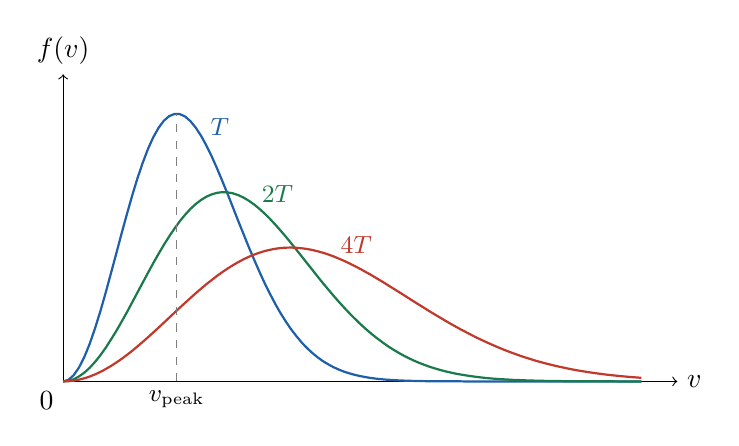
\begin{tikzpicture}
		\draw [->] (0,0) -- (7.8,0) node [right] {$v$};
		\draw [->] (0,0) -- (0,3.9) node [above] {$f(v)$};
		\draw [thick, mblue] plot coordinates {(0.000,0.000) (0.067,0.020) (0.135,0.080) (0.202,0.178) (0.270,0.312) (0.337,0.477) (0.404,0.671) (0.472,0.888) (0.539,1.122) (0.606,1.369) (0.674,1.621) (0.741,1.874) (0.809,2.121) (0.876,2.357) (0.943,2.577) (1.011,2.777) (1.078,2.953) (1.145,3.102) (1.213,3.222) (1.280,3.312) (1.348,3.370) (1.415,3.397) (1.482,3.395) (1.550,3.364) (1.617,3.305) (1.684,3.223) (1.752,3.119) (1.819,2.996) (1.887,2.858) (1.954,2.707) (2.021,2.547) (2.089,2.381) (2.156,2.211) (2.223,2.041) (2.291,1.872) (2.358,1.706) (2.426,1.546) (2.493,1.393) (2.560,1.247) (2.628,1.111) (2.695,0.983) (2.762,0.866) (2.830,0.758) (2.897,0.660) (2.965,0.572) (3.032,0.492) (3.099,0.422) (3.167,0.360) (3.234,0.305) (3.301,0.257) (3.369,0.216) (3.436,0.180) (3.504,0.149) (3.571,0.123) (3.638,0.102) (3.706,0.083) (3.773,0.068) (3.840,0.055) (3.908,0.044) (3.975,0.035) (4.043,0.028) (4.110,0.022) (4.177,0.018) (4.245,0.014) (4.312,0.011) (4.379,0.008) (4.447,0.007) (4.514,0.005) (4.582,0.004) (4.649,0.003) (4.716,0.002) (4.784,0.002) (4.851,0.001) (4.918,0.001) (4.986,0.001) (5.053,0.001) (5.121,0.000) (5.188,0.000) (5.255,0.000) (5.323,0.000) (5.390,0.000) (5.457,0.000) (5.525,0.000) (5.592,0.000) (5.660,0.000) (5.727,0.000) (5.794,0.000) (5.862,0.000) (5.929,0.000) (5.996,0.000) (6.064,0.000) (6.131,0.000) (6.199,0.000) (6.266,0.000) (6.333,0.000) (6.401,0.000) (6.468,0.000) (6.535,0.000) (6.603,0.000) (6.670,0.000) (6.738,0.000) (6.805,0.000) (6.872,0.000) (6.940,0.000) (7.007,0.000) (7.074,0.000) (7.142,0.000) (7.209,0.000) (7.277,0.000) (7.344,0.000)};
		\draw [thick, mgreen] plot coordinates {(0.000,0.000) (0.067,0.007) (0.135,0.028) (0.202,0.064) (0.270,0.112) (0.337,0.173) (0.404,0.247) (0.472,0.331) (0.539,0.425) (0.606,0.529) (0.674,0.639) (0.741,0.756) (0.809,0.877) (0.876,1.002) (0.943,1.128) (1.011,1.255) (1.078,1.380) (1.145,1.503) (1.213,1.622) (1.280,1.736) (1.348,1.843) (1.415,1.943) (1.482,2.035) (1.550,2.118) (1.617,2.191) (1.684,2.253) (1.752,2.305) (1.819,2.346) (1.887,2.376) (1.954,2.395) (2.021,2.404) (2.089,2.401) (2.156,2.389) (2.223,2.367) (2.291,2.335) (2.358,2.295) (2.426,2.247) (2.493,2.192) (2.560,2.131) (2.628,2.063) (2.695,1.991) (2.762,1.915) (2.830,1.836) (2.897,1.754) (2.965,1.670) (3.032,1.585) (3.099,1.500) (3.167,1.415) (3.234,1.330) (3.301,1.247) (3.369,1.166) (3.436,1.086) (3.504,1.009) (3.571,0.935) (3.638,0.864) (3.706,0.796) (3.773,0.731) (3.840,0.669) (3.908,0.611) (3.975,0.557) (4.043,0.506) (4.110,0.458) (4.177,0.414) (4.245,0.373) (4.312,0.335) (4.379,0.300) (4.447,0.268) (4.514,0.239) (4.582,0.213) (4.649,0.188) (4.716,0.167) (4.784,0.147) (4.851,0.129) (4.918,0.114) (4.986,0.099) (5.053,0.087) (5.121,0.076) (5.188,0.066) (5.255,0.057) (5.323,0.049) (5.390,0.042) (5.457,0.036) (5.525,0.031) (5.592,0.027) (5.660,0.023) (5.727,0.019) (5.794,0.017) (5.862,0.014) (5.929,0.012) (5.996,0.010) (6.064,0.008) (6.131,0.007) (6.199,0.006) (6.266,0.005) (6.333,0.004) (6.401,0.003) (6.468,0.003) (6.535,0.002) (6.603,0.002) (6.670,0.002) (6.738,0.001) (6.805,0.001) (6.872,0.001) (6.940,0.001) (7.007,0.001) (7.074,0.000) (7.142,0.000) (7.209,0.000) (7.277,0.000) (7.344,0.000)};
		\draw [thick, mred] plot coordinates {(0.000,0.000) (0.067,0.003) (0.135,0.010) (0.202,0.023) (0.270,0.040) (0.337,0.062) (0.404,0.089) (0.472,0.120) (0.539,0.156) (0.606,0.195) (0.674,0.239) (0.741,0.285) (0.809,0.336) (0.876,0.388) (0.943,0.444) (1.011,0.502) (1.078,0.561) (1.145,0.622) (1.213,0.684) (1.280,0.747) (1.348,0.811) (1.415,0.874) (1.482,0.937) (1.550,0.999) (1.617,1.060) (1.684,1.120) (1.752,1.178) (1.819,1.235) (1.887,1.288) (1.954,1.340) (2.021,1.388) (2.089,1.434) (2.156,1.476) (2.223,1.515) (2.291,1.551) (2.358,1.583) (2.426,1.611) (2.493,1.635) (2.560,1.656) (2.628,1.672) (2.695,1.685) (2.762,1.694) (2.830,1.699) (2.897,1.700) (2.965,1.697) (3.032,1.691) (3.099,1.682) (3.167,1.669) (3.234,1.653) (3.301,1.634) (3.369,1.612) (3.436,1.587) (3.504,1.559) (3.571,1.530) (3.638,1.498) (3.706,1.464) (3.773,1.429) (3.840,1.392) (3.908,1.354) (3.975,1.314) (4.043,1.274) (4.110,1.232) (4.177,1.190) (4.245,1.148) (4.312,1.106) (4.379,1.063) (4.447,1.020) (4.514,0.978) (4.582,0.936) (4.649,0.894) (4.716,0.853) (4.784,0.813) (4.851,0.773) (4.918,0.734) (4.986,0.696) (5.053,0.659) (5.121,0.624) (5.188,0.589) (5.255,0.555) (5.323,0.523) (5.390,0.492) (5.457,0.462) (5.525,0.433) (5.592,0.405) (5.660,0.379) (5.727,0.354) (5.794,0.330) (5.862,0.307) (5.929,0.286) (5.996,0.265) (6.064,0.246) (6.131,0.228) (6.199,0.211) (6.266,0.195) (6.333,0.180) (6.401,0.166) (6.468,0.152) (6.535,0.140) (6.603,0.129) (6.670,0.118) (6.738,0.108) (6.805,0.099) (6.872,0.090) (6.940,0.082) (7.007,0.075) (7.074,0.068) (7.142,0.062) (7.209,0.056) (7.277,0.051) (7.344,0.046)};
		\draw [dashed, gray] (1.442,0) -- (1.442,3.4);
		\node [mblue, above right] at (1.75,3.0) {\small $T$};
		\node [mgreen, above right] at (2.4,2.15) {\small $2T$};
		\node [mred, above right] at (3.4,1.5) {\small $4T$};
		\node [below] at (1.442,0) {\small $v_{\mathrm{peak}}$};
		\node [below left] at (0,0) {$0$};
	\end{tikzpicture}
\end{center}

Three different `average' speeds are in common use, and it is worth knowing that they differ. Alongside $v_{\mathrm{peak}} = \sqrt{2kT/m}$ we have the mean speed
$$
\avg v = \int_0^\infty v f(v) \dd v = \sqrt{\frac{8kT}{\pi m}},
$$
and the root-mean-square speed, which by equipartition satisfies $\tfrac 12 m \avg{v^2} = \tfrac 32 kT$, so
$$
v_{\mathrm{rms}} = \sqrt{\avg{v^2}} = \sqrt{\frac{3kT}{m}}.
$$
These are in the ratio $1 : \sqrt{4/\pi} : \sqrt{3/2} \approx 1 : 1.13 : 1.22$, in the order stated -- which is what one expects from a distribution with a long tail to the right.

\begin{example}
	For nitrogen ($m \approx 4.7\times 10^{-26}\,\mathrm{kg}$) at room temperature, $v_{\mathrm{rms}} \approx 500\,\mathrm{m}\,\mathrm{s}^{-1}$, comfortably faster than the speed of sound. Molecules in the air around you are moving very quickly indeed; they do not get very far, because they collide constantly.
\end{example}

\subsection{Indistinguishability and the Gibbs Paradox}\label{sec:gibbsparadox}

We must now return to the factor of $1/N!$ that we inserted without justification. Suppose we had not: take $Z = Z_1^N$, so that
$$
\log Z = N \log \frac{V}{\lambda^3}, \qquad S = Nk\left(\log\frac{V}{\lambda^3} + \frac 32\right).
$$
The pressure and energy are unaffected, but the entropy is wrong -- and wrong in an instructive way. Under $V \mapsto \lambda V$, $N \mapsto \lambda N$ this $S$ does not scale as $\lambda S$; it is not extensive. That is a disaster, since we argued in Section~1.11 that entropy must be extensive.

The physical version of this disaster is the following.

\begin{example}[Gibbs paradox]
	Take a box of volume $2V$ containing $2N$ molecules of the same gas at temperature $T$, and insert a partition down the middle, so we now have two boxes each of volume $V$ containing $N$ molecules. Using the non-extensive formula, the total entropy before was
	$$
	S_{\mathrm{before}} = 2Nk\left(\log\frac{2V}{\lambda^3} + \frac 32\right),
	$$
	and afterwards
	$$
	S_{\mathrm{after}} = 2 \times Nk\left(\log\frac{V}{\lambda^3} + \frac 32\right),
	$$
	so $S_{\mathrm{before}} - S_{\mathrm{after}} = 2Nk\log 2 > 0$. Removing the partition would then increase the entropy by $2Nk\log 2$. But nothing has happened! The gas is the same on both sides; inserting and removing a partition is completely reversible, and cannot change the entropy at all.
\end{example}

The resolution, due to Gibbs, is that we have over-counted. Two configurations differing only by swapping particle 1 with particle 2 are not different configurations, because the particles are \emph{identical}: there is no experiment that could distinguish them. When we integrated each particle independently over the box, we counted each genuine configuration $N!$ times, once for each way of labelling the particles. So we should divide by $N!$:
$$
Z = \frac{Z_1^N}{N!},
$$
which is what we assumed above and which gives the extensive Sackur--Tetrode entropy. Since $\log N! \approx N\log N - N$, the correction changes $S$ by $-Nk(\log N - 1)$, converting $\log(V/\lambda^3)$ into $\log(V/N\lambda^3)$ and curing the paradox: with the correct formula, $S_{\mathrm{before}} = S_{\mathrm{after}}$ exactly.

Two remarks. First, if the two halves contain \emph{different} gases, then removing the partition really does increase the entropy, by exactly $2Nk\log 2$; this is the \vocab{entropy of mixing}, and it is real, since unmixing two gases genuinely costs work. Secondly, and more strikingly: indistinguishability of identical particles is a quantum-mechanical fact. Classical particles could in principle be labelled and followed. So this is the second place where classical statistical mechanics needed to be rescued by quantum mechanics -- and the $1/N!$ is only an approximation to the correct quantum counting, valid when the chance of two particles occupying the same state is negligible. That is precisely the regime $\lambda^3 \ll V/N$ identified earlier.

\subsection{Diatomic Gases}

Real gases are usually not monatomic. A diatomic molecule can rotate and vibrate as well as translate, and each of these gives extra degrees of freedom. Since the different motions are (approximately) independent, the partition functions multiply:
$$
Z_1 = Z_{\mathrm{trans}} Z_{\mathrm{rot}} Z_{\mathrm{vib}}.
$$

The rotational degrees of freedom are the two angles specifying the axis of the molecule. Quantum mechanically, a rigid rotor has energy levels
$$
E_j = \frac{\hbar^2}{2I}j(j+1), \qquad j = 0, 1, 2, \dots
$$
with degeneracy $2j+1$, where $I$ is the moment of inertia. So
$$
Z_{\mathrm{rot}} = \sum_{j=0}^\infty (2j+1)e^{-\beta \hbar^2 j(j+1)/2I}.
$$
At high temperature, $kT \gg \hbar^2/2I$, the summand varies slowly and we may replace the sum by an integral; substituting $u = j(j+1)$, so $\dd u = (2j+1)\dd j$,
$$
Z_{\mathrm{rot}} \approx \int_0^\infty (2j+1)e^{-\beta\hbar^2 j(j+1)/2I}\dd j = \int_0^\infty e^{-\beta\hbar^2 u/2I}\dd u = \frac{2I}{\beta\hbar^2}.
$$
This gives $E_{\mathrm{rot}} = -\partial_\beta \log Z_{\mathrm{rot}} = kT$ per molecule, exactly as equipartition predicts for two quadratic degrees of freedom. At low temperature, $kT \ll \hbar^2/2I$, only the first two terms matter,
$$
Z_{\mathrm{rot}} \approx 1 + 3e^{-\beta\hbar^2/I},
$$
giving $E_{\mathrm{rot}} \approx (3\hbar^2/I)e^{-\beta\hbar^2/I}$, which is exponentially small: the rotational modes are frozen out, and contribute nothing to the heat capacity.

The vibrational mode is a harmonic oscillator of frequency $\omega$, with energy levels $E_n = \hbar\omega(n + \tfrac 12)$. This we can sum exactly, as a geometric series:
$$
Z_{\mathrm{vib}} = \sum_{n=0}^\infty e^{-\beta \hbar\omega(n + 1/2)} = \frac{e^{-\beta\hbar\omega/2}}{1 - e^{-\beta\hbar\omega}} = \frac{1}{2\sinh(\beta\hbar\omega/2)},
$$
so the mean vibrational energy per molecule is
$$
E_{\mathrm{vib}} = -\frac{\partial}{\partial\beta}\log Z_{\mathrm{vib}} = \frac{\hbar\omega}{2}\coth\left(\frac{\beta\hbar\omega}{2}\right) = \hbar\omega\left(\frac{1}{2} + \frac{1}{e^{\beta\hbar\omega}-1}\right).
$$
At high temperature this tends to $kT$, again as equipartition demands; at low temperature it tends to the zero-point energy $\tfrac 12 \hbar\omega$, with exponentially small corrections. We will meet this formula again, twice, in the next section.

Putting it together, the heat capacity of a diatomic gas rises in steps as we heat it: $\tfrac 32 Nk$ when only translations are active, $\tfrac 52 Nk$ once rotations unfreeze, and $\tfrac 72 Nk$ once vibrations do. For hydrogen the rotational scale is about $85\,\mathrm{K}$ and the vibrational scale about $6000\,\mathrm{K}$, so at room temperature we see the middle plateau -- and indeed the measured $C_V$ of hydrogen is close to $\tfrac 52 Nk$. The steps are unmistakable in the data, and are direct macroscopic evidence for the quantisation of energy levels.

\subsection{Interacting Gases and the Virial Expansion}

Real gas molecules attract each other at long range and repel at short range, and we would like to know how this modifies the ideal gas law. The strategy is perturbative: for a dilute gas the number density $N/V$ is small, and we expand in it.

\begin{definition}[Virial expansion]
	The \vocab{virial expansion} of an equation of state is
	$$
	\frac{p}{kT} = \frac NV + B_2(T)\frac{N^2}{V^2} + B_3(T)\frac{N^3}{V^3} + \cdots,
	$$
	whose coefficients $B_k(T)$ are the \vocab{virial coefficients}.
\end{definition}

The coefficients depend only on $T$, since $p/kT$ and $N/V$ are both intensive. Our goal is to compute $B_2$.

Suppose the particles interact through a pair potential $U(r)$ depending only on the separation. What does $U$ look like? At long range, two neutral atoms attract: although each has zero average electric dipole moment, a fluctuation giving atom 1 a dipole $p_1$ produces a field $E \sim p_1/r^3$, which induces a dipole $p_2 \propto p_1/r^3$ in atom 2, and the resulting energy is
$$
U \sim -p_2 E \sim -\frac{p_1^2}{r^6}.
$$
This is the \vocab{van der Waals interaction}, and it is attractive. At short range the electron clouds overlap and the Pauli principle produces a strong repulsion. A convenient phenomenological form combining the two is the \vocab{Lennard-Jones potential}
$$
U(r) = U_0\left[\left(\frac{r_0}{r}\right)^{12} - \left(\frac{r_0}{r}\right)^6\right],
$$
where the twelfth power is chosen mostly because it is the square of the sixth and hence easy to compute with.

\begin{center}
	\begin{tikzpicture}
		\draw [->] (0,0) -- (7.9,0) node [right] {$r$};
		\draw [->] (0,-1.3) -- (0,3.1) node [above] {$U(r)$};
		\draw [thick, mblue] plot coordinates {(1.846,2.800) (1.869,2.113) (1.892,1.549) (1.915,1.087) (1.938,0.708) (1.961,0.400) (1.984,0.149) (2.007,-0.053) (2.029,-0.216) (2.052,-0.345) (2.075,-0.446) (2.098,-0.525) (2.121,-0.585) (2.144,-0.630) (2.167,-0.661) (2.190,-0.682) (2.213,-0.694) (2.236,-0.700) (2.259,-0.699) (2.282,-0.694) (2.305,-0.685) (2.328,-0.673) (2.351,-0.659) (2.374,-0.643) (2.397,-0.626) (2.420,-0.608) (2.443,-0.590) (2.466,-0.570) (2.489,-0.551) (2.511,-0.532) (2.534,-0.513) (2.557,-0.494) (2.580,-0.476) (2.603,-0.457) (2.626,-0.440) (2.649,-0.422) (2.672,-0.406) (2.695,-0.390) (2.718,-0.374) (2.741,-0.359) (2.764,-0.344) (2.787,-0.330) (2.810,-0.317) (2.833,-0.304) (2.856,-0.291) (2.879,-0.279) (2.902,-0.268) (2.925,-0.257) (2.948,-0.247) (2.970,-0.237) (2.993,-0.227) (3.016,-0.218) (3.039,-0.209) (3.062,-0.200) (3.085,-0.192) (3.108,-0.185) (3.131,-0.177) (3.154,-0.170) (3.177,-0.163) (3.200,-0.157) (3.240,-0.146) (3.342,-0.123) (3.443,-0.103) (3.545,-0.087) (3.646,-0.074) (3.748,-0.063) (3.849,-0.054) (3.951,-0.046) (4.052,-0.040) (4.154,-0.034) (4.255,-0.030) (4.357,-0.026) (4.458,-0.023) (4.560,-0.020) (4.662,-0.017) (4.763,-0.015) (4.865,-0.013) (4.966,-0.012) (5.068,-0.011) (5.169,-0.009) (5.271,-0.008) (5.372,-0.007) (5.474,-0.007) (5.575,-0.006) (5.677,-0.005) (5.778,-0.005) (5.880,-0.004) (5.982,-0.004) (6.083,-0.004) (6.185,-0.003) (6.286,-0.003) (6.388,-0.003) (6.489,-0.002) (6.591,-0.002) (6.692,-0.002) (6.794,-0.002) (6.895,-0.002) (6.997,-0.002) (7.098,-0.001) (7.200,-0.001)};
		\draw [dashed, gray] (2.245,0) -- (2.245,-0.700);
		\node [circ, mblue] at (2.245,-0.700) {};
		\node [above right] at (2.000,0) {\small $r_0$};
		\node [below] at (2.245,0) {\small $2^{1/6}r_0$};
	\end{tikzpicture}
\end{center}

For calculations it is easier to idealise this into a \vocab{hard-core potential}: infinitely repulsive inside $r_0$, attractive outside,
$$
U(r) = \begin{cases} \infty & r < r_0,\\ -U_0(r_0/r)^6 & r \geq r_0.\end{cases}
$$
\begin{center}
	\begin{tikzpicture}
		\draw [->] (0,0) -- (7.9,0) node [right] {$r$};
		\draw [->] (0,-1.6) -- (0,2.4) node [above] {$U(r)$};
		\draw [thick, mblue] plot coordinates {(2.000,-1.200) (2.088,-0.926) (2.176,-0.723) (2.264,-0.570) (2.353,-0.453) (2.441,-0.363) (2.529,-0.294) (2.617,-0.239) (2.705,-0.196) (2.793,-0.162) (2.881,-0.134) (2.969,-0.112) (3.058,-0.094) (3.146,-0.079) (3.234,-0.067) (3.322,-0.057) (3.410,-0.049) (3.498,-0.042) (3.586,-0.036) (3.675,-0.031) (3.763,-0.027) (3.851,-0.024) (3.939,-0.021) (4.027,-0.018) (4.115,-0.016) (4.203,-0.014) (4.292,-0.012) (4.380,-0.011) (4.468,-0.010) (4.556,-0.009) (4.644,-0.008) (4.732,-0.007) (4.820,-0.006) (4.908,-0.005) (4.997,-0.005) (5.085,-0.004) (5.173,-0.004) (5.261,-0.004) (5.349,-0.003) (5.437,-0.003) (5.525,-0.003) (5.614,-0.002) (5.702,-0.002) (5.790,-0.002) (5.878,-0.002) (5.966,-0.002) (6.054,-0.002) (6.142,-0.001) (6.231,-0.001) (6.319,-0.001) (6.407,-0.001) (6.495,-0.001) (6.583,-0.001) (6.671,-0.001) (6.759,-0.001) (6.847,-0.001) (6.936,-0.001) (7.024,-0.001) (7.112,-0.001) (7.200,-0.001)};
		\draw [thick, mblue] (2.0,-1.2) -- (2.0,2.2);
		\node [above right] at (2.0,0) {\small $r_0$};
	\end{tikzpicture}
\end{center}

Now to the calculation. The Hamiltonian of the gas is
$$
H = \sum_{i=1}^N \frac{\vv p_i^2}{2m} + \sum_{i < j} U(r_{ij}), \qquad r_{ij} = |\vv r_i - \vv r_j|,
$$
and the partition function no longer factorises. The momentum integrals still do, however, and they give the same $\lambda^{-3N}$ as before:
$$
Z(N,V,T) = \frac{1}{N!\lambda^{3N}}\int \prod_i \dd^3 r_i \; e^{-\beta\sum_{j<k}U(r_{jk})}.
$$
We would now like to expand the exponential in powers of $U$, but this is hopeless: $U$ is infinite at short range. The trick is to expand instead in the \vocab{Mayer $f$-function}
$$
f(r) = e^{-\beta U(r)} - 1,
$$
which is well behaved: it equals $-1$ inside the hard core and tends to $0$ as $r \to \infty$, so it is supported on a shell of finite size. Writing $f_{jk} = f(r_{jk})$,
$$
e^{-\beta\sum_{j<k}U_{jk}} = \prod_{j<k}(1+f_{jk}) = 1 + \sum_{j<k}f_{jk} + \sum_{j<k}\sum_{\ell<m}f_{jk}f_{\ell m} + \cdots.
$$
The first term integrates to $V^N$, giving the ideal gas. Each term in the second sum gives, say for $j=1,k=2$,
$$
\int \prod_i \dd^3 r_i \; f_{12} = V^{N-2}\int \dd^3 r_1 \dd^3 r_2 \; f(r_{12}) = V^{N-1} I, \qquad I = \int \dd^3 r\; f(r),
$$
where we changed to relative and centre-of-mass coordinates and extended the $r$ integral over all space (legitimate since $f$ decays). There are $\binom N2 \approx N^2/2$ such terms, so
$$
Z = \frac{V^N}{N!\lambda^{3N}}\left(1 + \frac{N^2 I}{2V} + \cdots\right) = Z_{\mathrm{ideal}}\left(1 + \frac{NI}{2V}+\cdots\right)^N,
$$
where in the last step we pulled an $N$ into the exponent, which is legitimate to this order and has the advantage of making extensivity manifest. Then
$$
F = -kT\log Z = F_{\mathrm{ideal}} - NkT\log\left(1 + \frac{NI}{2V}+\cdots\right) \approx F_{\mathrm{ideal}} - \frac{N^2 kT}{2V}I,
$$
and differentiating,
$$
p = -\left(\frac{\partial F}{\partial V}\right)_T = \frac{NkT}{V}\left(1 - \frac{NI}{2V}+\cdots\right).
$$

\begin{proposition}
	The second virial coefficient is
	$$
	B_2(T) = -\frac 12 I = -\frac 12\int \dd^3 r \left(e^{-\beta U(r)}-1\right).
	$$
\end{proposition}

The expansion parameter is $NI/V$, and $I \sim r_0^3$, so we need $N/V \ll r_0^{-3}$: the gas must be much less dense than a liquid, which is exactly the regime in which we expect a dilute-gas expansion to work. Note also the sign: a purely repulsive potential has $U > 0$, hence $f < 0$, hence $B_2 > 0$, and the pressure is increased. A purely attractive potential decreases it. Both are what one would guess.

\subsection{The van der Waals Equation}\label{sec:vdwderive}

Let us evaluate $I$ for the hard-core potential. Splitting the integral at $r_0$,
$$
I = \int_{r<r_0}\dd^3 r\;(-1) + \int_{r>r_0}\dd^3 r\left(e^{\beta U_0 (r_0/r)^6}-1\right).
$$
The first piece is just $-\tfrac 43 \pi r_0^3$. For the second we assume high temperature, $\beta U_0 \ll 1$, and expand the exponential to first order:
$$
\int_{r_0}^\infty 4\pi r^2 \dd r\; \beta U_0 \frac{r_0^6}{r^6} = 4\pi \beta U_0 r_0^6 \int_{r_0}^\infty \frac{\dd r}{r^4} = \frac{4\pi r_0^3 U_0}{3kT}.
$$
Hence
$$
I = \frac{4\pi r_0^3}{3}\left(\frac{U_0}{kT}-1\right),
$$
and substituting into the virial expansion,
$$
\frac{pV}{NkT} = 1 - \frac NV\left(\frac{a}{kT}-b\right), \qquad a = \frac{2\pi r_0^3 U_0}{3}, \quad b = \frac{2\pi r_0^3}{3}.
$$
This is already a decent equation of state, but it is traditional (and, as we will see, far more useful) to rearrange it. Inverting,
$$
kT = \frac VN\left(p + \frac{aN^2}{V^2}\right)\left(1 + \frac{bN}{V}\right)^{-1} \approx \left(p + \frac{aN^2}{V^2}\right)\left(\frac VN - b\right),
$$
where we expanded the inverse to first order and discarded higher terms, which are beyond the accuracy we have anyway.

\begin{definition}[van der Waals equation]
	The \vocab{van der Waals equation of state} is
	$$
	\left(p + \frac{aN^2}{V^2}\right)\left(\frac VN - b\right) = kT, \qquad \text{equivalently} \qquad p = \frac{NkT}{V - bN} - \frac{aN^2}{V^2}.
	$$
\end{definition}

The second form makes the interpretation clear. The $b$ term says that the volume available to the gas is reduced, because the molecules take up room; the $a$ term says the pressure is reduced, because the long-range attraction pulls molecules back from the walls.

The factor of $bN$ deserves a comment, since it is not what one would first guess. Two hard spheres of core radius $r_0$ cannot approach closer than $r_0$, so each atom excludes a volume
$$
\Omega_{\mathrm{ex}} = \tfrac 43 \pi r_0^3 = 2b
$$
around itself -- twice the value of $b$. Why the factor of two? Because the exclusion is shared between pairs. Placing the atoms in one at a time, the first has volume $V$ available, the second $V - \Omega_{\mathrm{ex}}$, the third $V - 2\Omega_{\mathrm{ex}}$, and so on, so the accessible configuration volume is
$$
\frac{1}{N!}\prod_{j=0}^{N-1}\left(V - j\Omega_{\mathrm{ex}}\right) \approx \frac{V^N}{N!}\left(1 - \frac{N^2\Omega_{\mathrm{ex}}}{2V}\right) \approx \frac{1}{N!}\left(V - \frac{N\Omega_{\mathrm{ex}}}{2}\right)^N,
$$
so the effective excluded volume \emph{per particle} is $\Omega_{\mathrm{ex}}/2 = b$.

We derived the van der Waals equation in a regime where it is a small correction to the ideal gas law. Its real interest, though, is what happens if we take it seriously outside that regime -- where, as we will see in Section~\ref{sec:liquidgas}, it produces a liquid--gas phase transition. That is an entirely illegitimate extrapolation, and it works remarkably well.

Higher virial coefficients can be computed, but not by naively keeping the $\sum\sum f_{jk}f_{\ell m}$ terms; one has to be careful about which diagrams contribute at which order in $N/V$. The systematic method is the \vocab{cluster expansion}, which organises the terms into connected diagrams in a manner very reminiscent of Feynman diagrams. We will not pursue it.

\section{Quantum Gases}\label{sec:quantumgases}

We saw that the classical treatment of a gas should break down when the thermal wavelength $\lambda$ becomes comparable with the interparticle spacing, that is, when the gas is cold or dense. In this section we do the calculation properly. This is where statistical physics earns its keep: the same formalism will give us the spectrum of light from a hot object, the heat capacity of a crystal, the pressure that holds up a white dwarf star, and a phase transition with no interactions in sight.

The technical obstacle is that the partition function is a sum over states, and quantum states are discrete. In practice the levels are very finely spaced, so we would like to replace the sum by an integral -- but we must keep track of how many states there are per unit energy. That is the density of states.

\subsection{Density of States}\label{sec:dos}

Consider a single particle in a cubical box of side $L$, so $V = L^3$. The energy eigenstates are the standing waves
$$
\psi(\vv r) \propto \sin\left(\frac{n_1 \pi x}{L}\right)\sin\left(\frac{n_2\pi y}{L}\right)\sin\left(\frac{n_3 \pi z}{L}\right), \qquad n_i \in \N,
$$
though for counting purposes it is more convenient to use periodic boundary conditions, which give plane waves $e^{i\vv k \cdot \vv r}$ with
$$
\vv k = \frac{2\pi}{L}(n_1, n_2, n_3), \qquad n_i \in \Z.
$$
Either way the answer is the same: the allowed wavevectors form a lattice in $\vv k$-space with one state per volume $(2\pi/L)^3 = (2\pi)^3/V$. So for a large box the number of states with wavevector in $\dd^3 k$ is
$$
\frac{V}{(2\pi)^3}\dd^3 k,
$$
and equivalently, since $\vv p = \hbar \vv k$, one state per phase-space volume $(2\pi\hbar)^3$. This is exactly the normalisation we were forced to guess in Section~\ref{sec:classicalZ}, and now we have derived it.

Now specialise to a non-relativistic particle, $E = \hbar^2 k^2/2m$. Counting states with energy less than $E$ means counting lattice points inside a sphere of radius $k = \sqrt{2mE}/\hbar$:
$$
g(E)\dd E = \frac{V}{(2\pi)^3}\,4\pi k^2 \dd k = \frac{V}{2\pi^2}k^2 \frac{\dd k}{\dd E}\dd E.
$$
Since $k = \sqrt{2mE}/\hbar$ we have $\dd k/\dd E = \sqrt{2m}/(2\hbar\sqrt E)$, and so we obtain the following.

\begin{definition}[Density of states]
	The \vocab{density of states} $g(E)$ is defined so that $g(E)\dd E$ is the number of single-particle states with energy in $[E, E+\dd E]$. For a non-relativistic particle of mass $m$ in a box of volume $V$ in three dimensions,
	$$
	g(E) = \frac{V}{4\pi^2}\left(\frac{2m}{\hbar^2}\right)^{3/2}\sqrt E.
	$$
\end{definition}

\begin{center}
	\begin{tikzpicture}
		\draw [->] (0,0) -- (7.4,0) node [right] {$E$};
		\draw [->] (0,0) -- (0,3.7) node [above] {$g(E)$};
		\draw [thick, mblue] plot coordinates {(0.000,0.000) (0.117,0.431) (0.234,0.609) (0.351,0.746) (0.468,0.861) (0.585,0.963) (0.702,1.055) (0.819,1.139) (0.936,1.218) (1.053,1.292) (1.169,1.361) (1.286,1.428) (1.403,1.491) (1.520,1.552) (1.637,1.611) (1.754,1.667) (1.871,1.722) (1.988,1.775) (2.105,1.826) (2.222,1.877) (2.339,1.925) (2.456,1.973) (2.573,2.019) (2.690,2.065) (2.807,2.109) (2.924,2.153) (3.041,2.195) (3.158,2.237) (3.275,2.278) (3.392,2.318) (3.508,2.358) (3.625,2.397) (3.742,2.435) (3.859,2.473) (3.976,2.510) (4.093,2.547) (4.210,2.583) (4.327,2.619) (4.444,2.654) (4.561,2.689) (4.678,2.723) (4.795,2.757) (4.912,2.790) (5.029,2.823) (5.146,2.856) (5.263,2.888) (5.380,2.920) (5.497,2.951) (5.614,2.983) (5.731,3.014) (5.847,3.044) (5.964,3.074) (6.081,3.104) (6.198,3.134) (6.315,3.164) (6.432,3.193) (6.549,3.222) (6.666,3.250) (6.783,3.279) (6.900,3.307)};
		\node [mblue, right] at (5.6,3.15) {\small $\propto \sqrt E$};
		\node [below left] at (0,0) {$0$};
	\end{tikzpicture}
\end{center}

The $\sqrt E$ is worth remembering, as is the fact that it depends on the dispersion relation and the dimension. If the particles have spin, or some other internal degree of freedom with $g_s$ states, we simply multiply $g(E)$ by $g_s$. And for massless particles such as photons, where $E = \hbar\omega = \hbar c k$, the same counting gives
$$
g(E) \dd E = \frac{V}{2\pi^2}k^2\dd k = \frac{V E^2}{2\pi^2 \hbar^3 c^3}\dd E,
$$
so $g(E) \propto E^2$ instead.

As a first check, let us recompute the partition function of a classical ideal gas:
$$
Z_1 = \int_0^\infty \dd E\; g(E) e^{-\beta E} = \frac{V}{4\pi^2}\left(\frac{2m}{\hbar^2}\right)^{3/2}\int_0^\infty \sqrt E e^{-\beta E}\dd E = \frac{V}{4\pi^2}\left(\frac{2m}{\hbar^2}\right)^{3/2}\frac{\sqrt\pi}{2\beta^{3/2}} = \frac{V}{\lambda^3},
$$
agreeing with our earlier result.

\subsection{Blackbody Radiation}\label{sec:blackbody}

Our first application is to light. Consider an empty box whose walls are held at temperature $T$. The walls constantly emit and absorb photons, so the box fills with electromagnetic radiation in thermal equilibrium; this is \vocab{blackbody radiation}, and the question is what its spectrum looks like. The problem is a genuinely historic one -- getting it wrong is what started quantum mechanics.

The electromagnetic field in a box is equivalent to a collection of harmonic oscillators, one for each mode $(\vv k, \text{polarisation})$, with frequency $\omega = ck$. Quantum mechanically each oscillator has energy levels $E_n = \hbar\omega(n+\tfrac 12)$, and we interpret $n$ as the number of photons in that mode. Crucially, photon number is not conserved -- the walls create and destroy photons freely -- so there is no constraint on $n$, and we may compute the partition function of each mode separately. Discarding the zero-point energy (which is an infinite constant, and does not affect anything we measure here),
$$
Z_{\vv k} = \sum_{n=0}^\infty e^{-\beta n \hbar\omega} = \frac{1}{1 - e^{-\beta\hbar\omega}}.
$$
The mean number of photons in the mode is then
$$
\avg n = \frac{1}{Z_{\vv k}}\sum_{n\ge 0} n e^{-\beta n\hbar\omega} = -\frac{1}{\hbar}\frac{\partial \log Z_{\vv k}}{\partial\beta}\cdot\frac{1}{\omega},
$$
which evaluates to the following.

\begin{definition}[Planck distribution]
	The mean occupation number of a photon mode of frequency $\omega$ at temperature $T$ is
	$$
	\avg{n(\omega)} = \frac{1}{e^{\beta\hbar\omega}-1}.
	$$
\end{definition}

Now we sum over modes. There are two polarisations for each wavevector, so the number of modes with frequency in $[\omega, \omega+\dd\omega]$ is
$$
2 \cdot \frac{V}{(2\pi)^3}4\pi k^2 \dd k = \frac{V\omega^2}{\pi^2 c^3}\dd\omega,
$$
using $\omega = ck$. Multiplying by $\hbar\omega \avg{n(\omega)}$ gives the energy.

\begin{proposition}[Planck's law]
	The energy density of blackbody radiation per unit frequency is
	$$
	\frac{E(\omega)}{V} = \frac{\hbar}{\pi^2 c^3}\frac{\omega^3}{e^{\beta\hbar\omega}-1}.
	$$
\end{proposition}

Let us look at the two limits. For $\hbar\omega \ll kT$ we may expand $e^{\beta\hbar\omega} - 1 \approx \beta\hbar\omega$, giving
$$
\frac{E(\omega)}{V} \approx \frac{\omega^2 kT}{\pi^2 c^3},
$$
which is the \vocab{Rayleigh--Jeans law}. This is exactly what classical equipartition predicts: each mode is an oscillator with two quadratic degrees of freedom, hence energy $kT$, and there are $\omega^2 \dd\omega \,V/\pi^2c^3$ of them. It agrees beautifully with experiment at low frequencies, and it is a catastrophe at high ones -- the total energy $\int_0^\infty \omega^2 \dd\omega$ diverges. This is the \vocab{ultraviolet catastrophe}. Physically, the trouble is that there are infinitely many modes and classically every one of them must carry $kT$.

Quantum mechanics saves us. For $\hbar\omega \gg kT$ the Planck distribution is exponentially suppressed, $\avg n \approx e^{-\beta\hbar\omega}$: a mode whose quantum of energy exceeds $kT$ simply cannot be excited. The two behaviours are stitched together at $\hbar\omega \sim kT$, which is where the spectrum peaks.

\begin{center}
	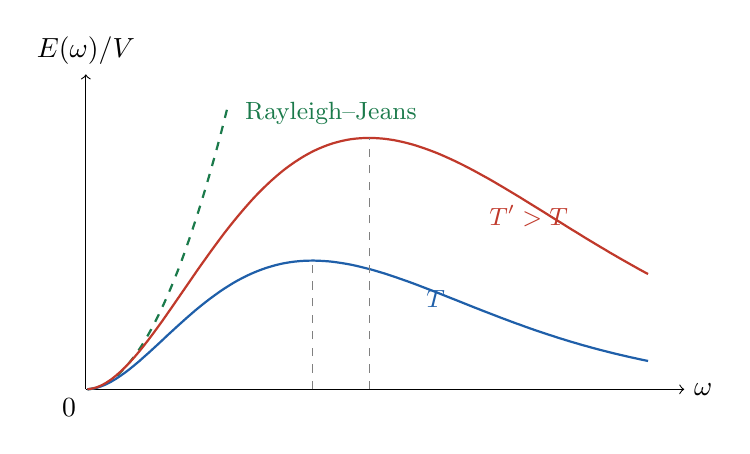
\begin{tikzpicture}
		\draw [->] (0,0) -- (7.6,0) node [right] {$\omega$};
		\draw [->] (0,0) -- (0,4.0) node [above] {$E(\omega)/V$};
		\draw [thick, dashed, mgreen] plot coordinates {(0.020,0.000) (0.066,0.005) (0.112,0.014) (0.158,0.028) (0.204,0.046) (0.250,0.069) (0.296,0.097) (0.342,0.129) (0.388,0.166) (0.433,0.208) (0.479,0.254) (0.525,0.305) (0.571,0.361) (0.617,0.421) (0.663,0.486) (0.709,0.555) (0.755,0.630) (0.801,0.709) (0.847,0.792) (0.892,0.880) (0.938,0.973) (0.984,1.071) (1.030,1.173) (1.076,1.280) (1.122,1.391) (1.168,1.507) (1.214,1.628) (1.260,1.754) (1.305,1.884) (1.351,2.019) (1.397,2.158) (1.443,2.302) (1.489,2.451) (1.535,2.604) (1.581,2.762) (1.627,2.925) (1.673,3.092) (1.719,3.264) (1.764,3.441) (1.810,3.623)};
		\draw [thick, mblue] plot coordinates {(0.020,0.000) (0.080,0.007) (0.140,0.020) (0.200,0.040) (0.260,0.065) (0.320,0.096) (0.379,0.131) (0.439,0.171) (0.499,0.213) (0.559,0.259) (0.619,0.308) (0.679,0.358) (0.738,0.411) (0.798,0.464) (0.858,0.519) (0.918,0.574) (0.978,0.630) (1.037,0.686) (1.097,0.741) (1.157,0.796) (1.217,0.850) (1.277,0.904) (1.337,0.956) (1.396,1.007) (1.456,1.056) (1.516,1.104) (1.576,1.150) (1.636,1.194) (1.696,1.237) (1.755,1.277) (1.815,1.315) (1.875,1.352) (1.935,1.386) (1.995,1.417) (2.055,1.447) (2.114,1.474) (2.174,1.499) (2.234,1.522) (2.294,1.543) (2.354,1.561) (2.414,1.578) (2.473,1.592) (2.533,1.604) (2.593,1.614) (2.653,1.622) (2.713,1.628) (2.773,1.632) (2.832,1.634) (2.892,1.635) (2.952,1.633) (3.012,1.630) (3.072,1.626) (3.131,1.620) (3.191,1.612) (3.251,1.603) (3.311,1.593) (3.371,1.582) (3.431,1.569) (3.490,1.555) (3.550,1.540) (3.610,1.525) (3.670,1.508) (3.730,1.490) (3.790,1.472) (3.849,1.453) (3.909,1.433) (3.969,1.412) (4.029,1.391) (4.089,1.370) (4.149,1.348) (4.208,1.326) (4.268,1.303) (4.328,1.280) (4.388,1.257) (4.448,1.234) (4.508,1.210) (4.567,1.186) (4.627,1.162) (4.687,1.139) (4.747,1.115) (4.807,1.091) (4.867,1.067) (4.926,1.043) (4.986,1.020) (5.046,0.996) (5.106,0.973) (5.166,0.950) (5.225,0.927) (5.285,0.904) (5.345,0.882) (5.405,0.859) (5.465,0.837) (5.525,0.816) (5.584,0.794) (5.644,0.773) (5.704,0.752) (5.764,0.732) (5.824,0.712) (5.884,0.692) (5.943,0.673) (6.003,0.653) (6.063,0.635) (6.123,0.616) (6.183,0.598) (6.243,0.581) (6.302,0.563) (6.362,0.547) (6.422,0.530) (6.482,0.514) (6.542,0.498) (6.602,0.483) (6.661,0.468) (6.721,0.453) (6.781,0.439) (6.841,0.425) (6.901,0.411) (6.961,0.398) (7.020,0.385) (7.080,0.372) (7.140,0.360)};
		\draw [thick, mred] plot coordinates {(0.020,0.001) (0.080,0.009) (0.140,0.026) (0.200,0.051) (0.260,0.084) (0.320,0.124) (0.379,0.171) (0.439,0.223) (0.499,0.281) (0.559,0.344) (0.619,0.411) (0.679,0.482) (0.738,0.556) (0.798,0.633) (0.858,0.713) (0.918,0.795) (0.978,0.878) (1.037,0.963) (1.097,1.049) (1.157,1.136) (1.217,1.223) (1.277,1.310) (1.337,1.397) (1.396,1.483) (1.456,1.569) (1.516,1.653) (1.576,1.737) (1.636,1.819) (1.696,1.900) (1.755,1.979) (1.815,2.056) (1.875,2.131) (1.935,2.204) (1.995,2.275) (2.055,2.344) (2.114,2.410) (2.174,2.474) (2.234,2.535) (2.294,2.593) (2.354,2.649) (2.414,2.702) (2.473,2.752) (2.533,2.800) (2.593,2.844) (2.653,2.886) (2.713,2.925) (2.773,2.962) (2.832,2.995) (2.892,3.026) (2.952,3.054) (3.012,3.079) (3.072,3.102) (3.131,3.122) (3.191,3.139) (3.251,3.154) (3.311,3.167) (3.371,3.177) (3.431,3.184) (3.490,3.189) (3.550,3.192) (3.610,3.193) (3.670,3.191) (3.730,3.187) (3.790,3.182) (3.849,3.174) (3.909,3.165) (3.969,3.153) (4.029,3.140) (4.089,3.125) (4.149,3.109) (4.208,3.091) (4.268,3.071) (4.328,3.050) (4.388,3.028) (4.448,3.005) (4.508,2.980) (4.567,2.954) (4.627,2.927) (4.687,2.899) (4.747,2.870) (4.807,2.840) (4.867,2.809) (4.926,2.778) (4.986,2.745) (5.046,2.712) (5.106,2.679) (5.166,2.645) (5.225,2.610) (5.285,2.575) (5.345,2.539) (5.405,2.503) (5.465,2.467) (5.525,2.431) (5.584,2.394) (5.644,2.357) (5.704,2.320) (5.764,2.283) (5.824,2.246) (5.884,2.208) (5.943,2.171) (6.003,2.134) (6.063,2.097) (6.123,2.059) (6.183,2.022) (6.243,1.986) (6.302,1.949) (6.362,1.912) (6.422,1.876) (6.482,1.840) (6.542,1.804) (6.602,1.769) (6.661,1.733) (6.721,1.699) (6.781,1.664) (6.841,1.630) (6.901,1.596) (6.961,1.562) (7.020,1.529) (7.080,1.496) (7.140,1.464)};
		\draw [dashed, gray] (2.878,0) -- (2.878,1.635);
		\draw [dashed, gray] (3.597,0) -- (3.597,3.193);
		\node [mgreen, right] at (1.9,3.5) {\small Rayleigh--Jeans};
		\node [mblue, right] at (4.2,1.15) {\small $T$};
		\node [mred, right] at (5.0,2.2) {\small $T' > T$};
		\node [below left] at (0,0) {$0$};
	\end{tikzpicture}
\end{center}

Two classical results drop out immediately. Differentiating Planck's law shows that the peak sits at $\hbar\omega_{\max} \approx 2.82\, kT$, so
$$
\omega_{\max} \propto T,
$$
which is \vocab{Wien's displacement law} -- the reason a heated poker glows first red and then white. And integrating over all frequencies, with $x = \beta\hbar\omega$,
$$
\frac EV = \frac{\hbar}{\pi^2c^3}\int_0^\infty \frac{\omega^3 \dd\omega}{e^{\beta\hbar\omega}-1} = \frac{(kT)^4}{\pi^2c^3\hbar^3}\int_0^\infty \frac{x^3\dd x}{e^x - 1} = \frac{\pi^2 k^4}{15 c^3\hbar^3}T^4,
$$
where we used $\int_0^\infty x^3/(e^x-1)\dd x = \pi^4/15$. This $T^4$ dependence is the \vocab{Stefan--Boltzmann law}. (To evaluate the integral, expand $1/(e^x-1) = \sum_{n\ge1}e^{-nx}$ and integrate term by term to get $\Gamma(4)\zeta(4) = 6\cdot \pi^4/90$.)

It is worth noting the whole thermodynamics of the photon gas. From
$$
\log \mathcal Z = -\sum_{\vv k, \text{pol}} \log\left(1 - e^{-\beta\hbar\omega}\right) = -\frac{V}{\pi^2c^3}\int_0^\infty \omega^2 \log\left(1-e^{-\beta\hbar\omega}\right)\dd\omega,
$$
an integration by parts gives $\log\mathcal Z = \beta E/3$, and hence, since $F = -kT\log \mathcal Z$ and $p = -(\partial F/\partial V)_T$,
$$
pV = \frac 13 E.
$$
This is the equation of state of \emph{radiation}, and the factor of $\tfrac 13$ (as opposed to $\tfrac 23$ for a non-relativistic gas, from $pV = NkT$ and $E = \tfrac 32 NkT$) is a general feature of ultrarelativistic gases. The entropy is $S = \tfrac 43 (E/T) \propto VT^3$.

\subsection{Phonons and the Debye Model}\label{sec:debye}

We turn to the heat capacity of a solid. Classically, by equipartition, a crystal of $N$ atoms is $3N$ oscillators and should have $C = 3Nk$ at all temperatures; experimentally $C \to 0$ as $T \to 0$, and in insulators it does so like $T^3$. The resolution is the same as for blackbody radiation, and the two calculations are almost identical.

The first attempt is due to Einstein: treat the solid as $3N$ independent oscillators, all of the same frequency $\omega$. Then, from our earlier computation of the vibrational partition function,
$$
E = 3N\hbar\omega\left(\frac 12 + \frac{1}{e^{\beta\hbar\omega}-1}\right), \qquad C = 3Nk\,(\beta\hbar\omega)^2 \frac{e^{\beta\hbar\omega}}{(e^{\beta\hbar\omega}-1)^2}.
$$
At high temperature this gives $C \to 3Nk$, recovering Dulong--Petit. At low temperature it gives $C \sim 3Nk(\beta\hbar\omega)^2 e^{-\beta\hbar\omega}$, which does vanish -- but exponentially, whereas experiment says $T^3$. Einstein's model has the right idea and the wrong details.

The flaw is the assumption that the oscillators are independent and identical. In reality the atoms are coupled, and the normal modes of the crystal are sound waves, with a range of frequencies. The quanta of these waves are called \vocab{phonons}, and they are treated exactly like photons: a mode of frequency $\omega$ has mean occupation $(e^{\beta\hbar\omega}-1)^{-1}$, and the number of phonons is not conserved.

\begin{definition}[Debye model]
	In the \vocab{Debye model} we assume a linear dispersion relation $\omega = c_s k$ for the sound waves, with $c_s$ the speed of sound, and we cut the spectrum off at a maximum frequency $\omega_D$ chosen so that the total number of modes is $3N$.
\end{definition}

The cutoff is not a fudge: a crystal of $N$ atoms has exactly $3N$ degrees of freedom, so there cannot be more than $3N$ modes. There are three polarisations (two transverse, one longitudinal), so
$$
3N = 3\cdot \frac{V}{(2\pi)^3}\int_{k < k_D}\dd^3 k = \frac{V k_D^3}{2\pi^2} \implies \omega_D = c_s\left(\frac{6\pi^2 N}{V}\right)^{1/3}.
$$
The energy is then, exactly as for photons but with three polarisations and a cutoff,
$$
E = \frac{3V}{2\pi^2c_s^3}\int_0^{\omega_D} \dd\omega\; \frac{\hbar\omega^3}{e^{\beta\hbar\omega}-1},
$$
dropping the zero-point contribution. Substituting $x = \beta\hbar\omega$ and defining the \vocab{Debye temperature} $T_D$ by $kT_D = \hbar\omega_D$,
$$
E = \frac{3V (kT)^4}{2\pi^2 c_s^3\hbar^3}\int_0^{T_D/T}\frac{x^3\dd x}{e^x - 1} = 9NkT\left(\frac{T}{T_D}\right)^3\int_0^{T_D/T}\frac{x^3\dd x}{e^x-1}.
$$
Now take the two limits.

For $T \gg T_D$ the upper limit is small, so $e^x - 1 \approx x$ and the integral is $\tfrac 13 (T_D/T)^3$, giving $E = 3NkT$ and $C = 3Nk$: Dulong--Petit, as it must be.

For $T \ll T_D$ the upper limit is effectively infinite, and the integral becomes the constant $\pi^4/15$. Hence
$$
E \approx \frac{3\pi^4}{5}NkT\left(\frac{T}{T_D}\right)^3, \qquad C \approx \frac{12\pi^4}{5}Nk\left(\frac{T}{T_D}\right)^3.
$$

\begin{proposition}[Debye $T^3$ law]
	At low temperatures the phonon contribution to the heat capacity of a solid is
	$$
	C = \frac{12\pi^4}{5}Nk\left(\frac{T}{T_D}\right)^3 \propto T^3.
	$$
\end{proposition}

This agrees with experiment. Here are the two models plotted together, in units where $C \to 3Nk$ at high temperature.

\begin{center}
	\begin{tikzpicture}
		\draw [->] (0,0) -- (7.2,0) node [right] {$T/T_D$};
		\draw [->] (0,0) -- (0,3.9) node [above] {$C/3Nk$};
		\draw [dashed, gray] (0,3.200) -- (7.0,3.200);
		\node [left] at (0,3.200) {$1$};
		\draw [thick, mblue] plot coordinates {(0.084,0.002) (0.159,0.013) (0.233,0.043) (0.308,0.098) (0.382,0.185) (0.457,0.306) (0.531,0.456) (0.606,0.625) (0.680,0.803) (0.755,0.982) (0.830,1.156) (0.904,1.321) (0.979,1.474) (1.053,1.616) (1.128,1.745) (1.202,1.862) (1.277,1.968) (1.352,2.064) (1.426,2.150) (1.501,2.228) (1.575,2.299) (1.650,2.363) (1.724,2.420) (1.799,2.473) (1.873,2.521) (1.948,2.564) (2.023,2.604) (2.097,2.640) (2.172,2.673) (2.246,2.704) (2.321,2.732) (2.395,2.757) (2.470,2.781) (2.545,2.803) (2.619,2.824) (2.694,2.842) (2.768,2.860) (2.843,2.876) (2.917,2.891) (2.992,2.906) (3.066,2.919) (3.141,2.931) (3.216,2.943) (3.290,2.954) (3.365,2.964) (3.439,2.974) (3.514,2.983) (3.588,2.991) (3.663,2.999) (3.738,3.007) (3.812,3.014) (3.887,3.021) (3.961,3.027) (4.036,3.033) (4.110,3.039) (4.185,3.044) (4.259,3.050) (4.334,3.055) (4.409,3.059) (4.483,3.064) (4.558,3.068) (4.632,3.072) (4.707,3.076) (4.781,3.080) (4.856,3.083) (4.931,3.087) (5.005,3.090) (5.080,3.093) (5.154,3.096) (5.229,3.099) (5.303,3.102) (5.378,3.104) (5.452,3.107) (5.527,3.109) (5.602,3.112) (5.676,3.114) (5.751,3.116) (5.825,3.118) (5.900,3.120) (5.974,3.122) (6.049,3.124) (6.124,3.126) (6.198,3.128) (6.273,3.129) (6.347,3.131) (6.422,3.133) (6.496,3.134) (6.571,3.136) (6.645,3.137) (6.720,3.138)};
		\draw [thick, mred] plot coordinates {(0.084,0.000) (0.159,0.000) (0.233,0.001) (0.308,0.012) (0.382,0.057) (0.457,0.154) (0.531,0.301) (0.606,0.483) (0.680,0.683) (0.755,0.886) (0.830,1.083) (0.904,1.269) (0.979,1.439) (1.053,1.595) (1.128,1.735) (1.202,1.860) (1.277,1.973) (1.352,2.074) (1.426,2.164) (1.501,2.245) (1.575,2.317) (1.650,2.382) (1.724,2.441) (1.799,2.494) (1.873,2.542) (1.948,2.585) (2.023,2.625) (2.097,2.661) (2.172,2.693) (2.246,2.723) (2.321,2.751) (2.395,2.776) (2.470,2.799) (2.545,2.821) (2.619,2.841) (2.694,2.859) (2.768,2.876) (2.843,2.892) (2.917,2.906) (2.992,2.920) (3.066,2.933) (3.141,2.945) (3.216,2.956) (3.290,2.966) (3.365,2.976) (3.439,2.985) (3.514,2.994) (3.588,3.002) (3.663,3.010) (3.738,3.017) (3.812,3.024) (3.887,3.030) (3.961,3.037) (4.036,3.042) (4.110,3.048) (4.185,3.053) (4.259,3.058) (4.334,3.063) (4.409,3.067) (4.483,3.072) (4.558,3.076) (4.632,3.079) (4.707,3.083) (4.781,3.087) (4.856,3.090) (4.931,3.093) (5.005,3.096) (5.080,3.099) (5.154,3.102) (5.229,3.105) (5.303,3.108) (5.378,3.110) (5.452,3.112) (5.527,3.115) (5.602,3.117) (5.676,3.119) (5.751,3.121) (5.825,3.123) (5.900,3.125) (5.974,3.127) (6.049,3.129) (6.124,3.130) (6.198,3.132) (6.273,3.134) (6.347,3.135) (6.422,3.137) (6.496,3.138) (6.571,3.139) (6.645,3.141) (6.720,3.142)};
		\node [mblue, below right] at (2.5,2.55) {\small Debye};
		\node [mred, right] at (2.2,1.75) {\small Einstein};
		\draw [dashed, gray] (4.200,0) -- (4.200,2.55);
		\node [below] at (4.200,0) {\small $1$};
		\node [below left] at (0,0) {$0$};
	\end{tikzpicture}
\end{center}

Both curves saturate at the classical value, and both vanish at $T=0$; the difference is in \emph{how} they vanish, and it is the low-temperature behaviour that distinguishes them. Physically, the Debye model works because there are always arbitrarily low-frequency sound waves available -- long-wavelength modes -- so however cold the solid, some modes can still be excited. The Einstein model has an energy gap, and so it is exponentially frozen.

\subsection{The Quantum Ideal Gas}

We now return to gases of massive particles, and do the counting properly. The key fact is quantum statistics: identical particles come in two kinds.

\begin{itemize}
	\item \vocab{Bosons}, which have integer spin, and for which any number of particles may occupy the same single-particle state.
	\item \vocab{Fermions}, which have half-integer spin, and for which the Pauli exclusion principle allows at most one particle per state.
\end{itemize}

Consider an ideal gas whose single-particle states are labelled by $r$ with energies $E_r$. A microstate of the whole gas is specified by the \vocab{occupation numbers} $\{n_r\}$, with total energy $\sum_r n_r E_r$ and total particle number $\sum_r n_r$. In the canonical ensemble, computing $Z = \sum_{\{n_r\}} e^{-\beta\sum n_r E_r}$ subject to $\sum_r n_r = N$ is horrible, because of the constraint. In the grand canonical ensemble the constraint disappears, and everything factorises:
$$
\mathcal Z = \sum_{\{n_r\}}e^{-\beta\sum_r n_r(E_r - \mu)} = \prod_r \left(\sum_{n_r} e^{-\beta n_r (E_r-\mu)}\right) = \prod_r \mathcal Z_r.
$$
This is exactly why we built the grand canonical ensemble, and the calculation is now easy.

For bosons the inner sum runs over all $n_r \ge 0$ and is geometric:
$$
\mathcal Z_r = \sum_{n=0}^\infty e^{-\beta n(E_r - \mu)} = \frac{1}{1 - e^{-\beta(E_r-\mu)}},
$$
which converges only if $\mu < E_r$ for every $r$; in particular $\mu$ must lie below the ground state energy, which we take to be $0$, so $\mu < 0$ for bosons. For fermions the sum has just two terms:
$$
\mathcal Z_r = 1 + e^{-\beta(E_r-\mu)}.
$$
The mean occupation of a state is $\avg{n_r} = -\beta^{-1}\partial \log\mathcal Z_r/\partial E_r$, and we obtain the two central distributions of the subject.

\begin{proposition}[Bose--Einstein and Fermi--Dirac distributions]
	The mean occupation number of a single-particle state of energy $E$ in an ideal quantum gas at temperature $T$ and chemical potential $\mu$ is
	$$
	\avg{n(E)} = \frac{1}{e^{\beta(E-\mu)}\mp 1},
	$$
	with the upper sign for bosons (\vocab{Bose--Einstein statistics}) and the lower for fermions (\vocab{Fermi--Dirac statistics}).
\end{proposition}

Some sanity checks. For fermions, $\avg n$ lies between $0$ and $1$, as the Pauli principle demands. For bosons, $\avg n$ diverges as $E \to \mu$, which is the seed of Bose--Einstein condensation. And when $e^{\beta(E-\mu)} \gg 1$ -- that is, when occupation numbers are small -- both reduce to
$$
\avg{n(E)} \approx e^{-\beta(E-\mu)},
$$
the classical Boltzmann distribution. So classical statistics is the dilute limit of both, as it should be. Setting $\mu = 0$ in the boson formula recovers the Planck distribution: photons are bosons whose number is not conserved, and a non-conserved particle number means exactly that there is no constraint to impose and hence $\mu = 0$.

Everything else follows. Converting sums to integrals with the density of states,
$$
N = \int_0^\infty \dd E\; \frac{g(E)}{e^{\beta(E-\mu)}\mp 1}, \qquad E_{\mathrm{tot}} = \int_0^\infty \dd E\; \frac{E\,g(E)}{e^{\beta(E-\mu)}\mp 1},
$$
and the grand potential is
$$
\Phi = -kT\log \mathcal Z = \pm kT \int_0^\infty \dd E\; g(E)\log\left(1 \mp e^{-\beta(E-\mu)}\right).
$$
Using $g(E) \propto E^{1/2}$ and integrating by parts gives a relation that holds for both statistics and will be useful repeatedly:
$$
pV = -\Phi = \frac 23 E_{\mathrm{tot}}.
$$

Before specialising, it is worth recording the classical limit as a criterion. In the dilute regime $N = \int g(E)e^{-\beta(E-\mu)}\dd E = e^{\beta\mu} V/\lambda^3$, so
$$
e^{\beta\mu} = \frac{N\lambda^3}{V}.
$$
The classical approximation required $e^{\beta\mu} \ll 1$, i.e.\ $\lambda^3 \ll V/N$, which is exactly the condition we anticipated. Quantum statistics matters when $\lambda^3 N/V \gtrsim 1$.

\subsection{Bosons and Bose--Einstein Condensation}\label{sec:bec}

Take a gas of $N$ non-relativistic bosons of mass $m$ and spin zero in a box of volume $V$, and fix $N$ by choosing $\mu$ appropriately:
$$
\frac NV = \frac{1}{4\pi^2}\left(\frac{2m}{\hbar^2}\right)^{3/2}\int_0^\infty \dd E\; \frac{\sqrt E}{z^{-1}e^{\beta E}-1}, \qquad z = e^{\beta\mu}.
$$
Substituting $x = \beta E$ and tidying up, this becomes
$$
\frac{N\lambda^3}{V} = g_{3/2}(z), \qquad \text{where} \quad g_{3/2}(z) = \frac{2}{\sqrt\pi}\int_0^\infty \frac{x^{1/2}\dd x}{z^{-1}e^x - 1}.
$$
The function $g_{3/2}$ has a nice series expansion: writing $\frac{1}{z^{-1}e^x-1} = \sum_{n\ge 1}z^n e^{-nx}$ and integrating term by term,
$$
g_{3/2}(z) = \sum_{n=1}^\infty \frac{z^n}{n^{3/2}}.
$$
This is manifestly increasing in $z$ on $0 \le z \le 1$, and recall that $\mu < 0$, so $z \le 1$. Hence $g_{3/2}$ attains its \emph{maximum} at $z = 1$:
$$
g_{3/2}(1) = \zeta(3/2) \approx 2.612.
$$
And now we have a problem. The left-hand side $N\lambda^3/V$ grows without bound as we cool the gas, since $\lambda \propto T^{-1/2}$. The right-hand side is bounded by $2.612$. So below a certain temperature the equation has no solution at all.

\begin{definition}[Critical temperature]
	The \vocab{critical temperature} for Bose--Einstein condensation is the temperature $T_c$ at which $N\lambda^3/V = \zeta(3/2)$, namely
	$$
	kT_c = \frac{2\pi\hbar^2}{m}\left(\frac{N}{\zeta(3/2)V}\right)^{2/3}.
	$$
\end{definition}

Something has gone wrong with our approximations, and it is easy to see what. In replacing the sum over states by an integral, we weighted the ground state $E=0$ by $g(0) = 0$ -- we threw it away. Usually this is harmless, since a single state out of $10^{23}$ cannot matter. But as $z \to 1$ the ground state occupation
$$
n_0 = \frac{1}{z^{-1}-1} = \frac{z}{1-z}
$$
diverges, and it can be macroscopically large. The resolution is to put the ground state back by hand:
$$
N = n_0 + \frac{V}{\lambda^3}g_{3/2}(z),
$$
where the integral now accounts for the excited states only. For $T > T_c$ we can solve for $z < 1$ with $n_0$ negligible. For $T < T_c$ the excited states can only hold
$$
N_{\mathrm{ex}} = \frac{V}{\lambda^3}\zeta(3/2) = N\left(\frac{T}{T_c}\right)^{3/2}
$$
particles, using $\lambda \propto T^{-1/2}$ and the definition of $T_c$; and the rest have nowhere to go but the ground state.

\begin{proposition}[Bose--Einstein condensation]
	For $T < T_c$, a macroscopic fraction of the particles occupies the single-particle ground state:
	$$
	\frac{n_0}{N} = 1 - \left(\frac{T}{T_c}\right)^{3/2}.
	$$
	This macroscopically occupied ground state is called the \vocab{Bose--Einstein condensate}.
\end{proposition}

\begin{center}
	\begin{tikzpicture}
		\draw [->] (0,0) -- (6.4,0) node [right] {$T$};
		\draw [->] (0,0) -- (0,3.6) node [above] {$n_0/N$};
		\draw [thick, mblue] plot coordinates {(0.000,3.000) (0.061,2.993) (0.122,2.981) (0.183,2.966) (0.244,2.947) (0.305,2.926) (0.366,2.903) (0.427,2.877) (0.488,2.850) (0.549,2.821) (0.610,2.791) (0.671,2.758) (0.732,2.725) (0.793,2.690) (0.854,2.653) (0.915,2.615) (0.976,2.576) (1.037,2.536) (1.098,2.494) (1.159,2.452) (1.220,2.408) (1.281,2.363) (1.342,2.317) (1.403,2.270) (1.464,2.222) (1.525,2.173) (1.586,2.122) (1.647,2.071) (1.708,2.019) (1.769,1.966) (1.831,1.912) (1.892,1.857) (1.953,1.802) (2.014,1.745) (2.075,1.688) (2.136,1.629) (2.197,1.570) (2.258,1.510) (2.319,1.449) (2.380,1.388) (2.441,1.325) (2.502,1.262) (2.563,1.198) (2.624,1.133) (2.685,1.068) (2.746,1.002) (2.807,0.935) (2.868,0.867) (2.929,0.799) (2.990,0.729) (3.051,0.660) (3.112,0.589) (3.173,0.518) (3.234,0.446) (3.295,0.373) (3.356,0.300) (3.417,0.226) (3.478,0.151) (3.539,0.076) (3.600,0.000)};
		\draw [thick, mblue] plot coordinates {(3.600,0.000) (5.580,0.000)};
		\draw [dashed, gray] (0,3.000) -- (1.0,3.000);
		\node [left] at (0,3.000) {$1$};
		\node [below] at (3.600,0) {$T_c$};
		\draw [dashed, gray] (3.600,0) -- (3.600,0.5);
		\node [below left] at (0,0) {$0$};
	\end{tikzpicture}
\end{center}

Note the shape: the condensate fraction rises from zero at $T_c$ with infinite slope (as $(T_c-T)^{1/2}$ near the transition... in fact as $\tfrac 32 (1 - T/T_c)$ to leading order, so with finite slope $3/2$), and reaches $1$ at $T = 0$. The chemical potential, meanwhile, is negative above $T_c$ and pinned to zero below it:

\begin{center}
	\begin{tikzpicture}
		\draw [->] (0,-1.5) -- (6.4,-1.5) node [right] {$T$};
		\draw [->] (0,-1.5) -- (0,0.9) node [above] {$\mu$};
		\draw [thick, mblue] plot coordinates {(0.000,0.000) (3.600,0.000)};
		\draw [thick, mblue] plot coordinates {(3.643,-0.000) (3.691,-0.002) (3.739,-0.004) (3.788,-0.007) (3.836,-0.011) (3.884,-0.016) (3.932,-0.022) (3.980,-0.028) (4.028,-0.036) (4.076,-0.044) (4.124,-0.053) (4.172,-0.062) (4.221,-0.073) (4.269,-0.084) (4.317,-0.096) (4.365,-0.108) (4.413,-0.122) (4.461,-0.136) (4.509,-0.150) (4.557,-0.166) (4.605,-0.182) (4.653,-0.198) (4.702,-0.216) (4.750,-0.233) (4.798,-0.252) (4.846,-0.271) (4.894,-0.291) (4.942,-0.311) (4.990,-0.332) (5.038,-0.353) (5.086,-0.375) (5.135,-0.398) (5.183,-0.421) (5.231,-0.445) (5.279,-0.469) (5.327,-0.493) (5.375,-0.519) (5.423,-0.544) (5.471,-0.570) (5.519,-0.597) (5.568,-0.624) (5.616,-0.652) (5.664,-0.680) (5.712,-0.709) (5.760,-0.738)};
		\node [below] at (3.600,-1.5) {$T_c$};
		\draw [dashed, gray] (3.600,-1.5) -- (3.600,0);
		\node [above left] at (0,0) {$0$};
	\end{tikzpicture}
\end{center}

What is remarkable about this is that it is a genuine phase transition -- a discontinuity in the derivative of a thermodynamic function -- occurring in a gas of \emph{non-interacting} particles. It is driven purely by quantum statistics. Physically, the condition $N\lambda^3/V \sim 1$ says the transition happens when the thermal wavelengths of the particles begin to overlap, at which point they can no longer be thought of as separate objects.

The thermodynamics below $T_c$ is easy, because the condensate contributes nothing to the energy (its particles have $E = 0$) or the pressure. Setting $z = 1$,
$$
E = \frac{V}{\lambda^3}kT\cdot \frac 32 g_{5/2}(1), \qquad g_{5/2}(1) = \zeta(5/2)\approx 1.342,
$$
so, using $\lambda \propto T^{-1/2}$, we get $E \propto V T^{5/2}$ and hence
$$
C_V = \left(\frac{\partial E}{\partial T}\right)_V \propto V T^{3/2}.
$$
So the heat capacity vanishes as $T^{3/2}$, in contrast to the classical constant $\tfrac 32 Nk$. Moreover $p = \tfrac 23 E/V \propto T^{5/2}$ is independent of $V$ -- if we compress a condensate at fixed temperature, the pressure does not rise, because the extra particles simply join the condensate. This is precisely analogous to the behaviour of a vapour in equilibrium with its liquid, and it is one of several respects in which the condensate behaves like a separate phase.

\begin{example}[Superfluid helium]
	Liquid ${}^4$He, whose atoms are bosons, undergoes a transition at $2.17\,\mathrm{K}$ below which it becomes a \vocab{superfluid}: it flows without viscosity, creeps up the walls of its container, and conducts heat extraordinarily well. Putting the density of liquid helium into our formula gives $T_c \approx 3.1\,\mathrm{K}$, which is the right order of magnitude -- encouraging, given that liquid helium is a strongly interacting system and our calculation assumed no interactions at all. By contrast ${}^3$He, whose atoms are fermions, shows no such transition at these temperatures (it does become superfluid, but at $2.5\,\mathrm{mK}$, and by a quite different mechanism involving pairs of atoms).
\end{example}

\subsection{Fermions and the Degenerate Fermi Gas}\label{sec:fermi}

Now the other case. For fermions the occupation function is
$$
\avg{n(E)} = \frac{1}{e^{\beta(E-\mu)}+1},
$$
and there is no convergence constraint on $\mu$, which may be positive or negative. The behaviour at low temperature is completely different from the bosonic case, and is dominated by the exclusion principle.

Consider first $T = 0$ exactly. Then $\beta \to \infty$, and
$$
\avg{n(E)} \to \begin{cases}1 & E < \mu,\\ 0 & E > \mu.\end{cases}
$$
So the particles fill up the energy levels from the bottom, one per state, until they run out. This is exactly what one would expect from the Pauli principle.

\begin{definition}[Fermi energy]
	The \vocab{Fermi energy} $E_F$ is the chemical potential at zero temperature, $E_F = \mu(T=0)$; equivalently, it is the energy of the highest occupied state at $T=0$. The corresponding momentum $k_F = \sqrt{2mE_F}/\hbar$ is the \vocab{Fermi momentum}, and the sphere $|\vv k| = k_F$ in momentum space is the \vocab{Fermi surface}.
\end{definition}

We can compute $E_F$ by counting. For spin-$\tfrac 12$ fermions there are two states per wavevector, so
$$
N = 2\cdot\frac{V}{(2\pi)^3}\cdot\frac 43 \pi k_F^3 = \frac{Vk_F^3}{3\pi^2} \implies E_F = \frac{\hbar^2}{2m}\left(\frac{3\pi^2 N}{V}\right)^{2/3}.
$$
The total energy at $T=0$ is
$$
E_{\mathrm{tot}} = \int_0^{E_F}E\, g(E)\dd E = \frac 35 N E_F,
$$
using $g(E) \propto \sqrt E$, and hence, by the relation $pV = \tfrac 23 E_{\mathrm{tot}}$,
$$
p = \frac{2NE_F}{5V} \propto \left(\frac NV\right)^{5/3}.
$$
This is \vocab{degeneracy pressure}, and it is a purely quantum effect: a Fermi gas at absolute zero exerts an enormous pressure, not because the particles are hot, but because they cannot all sit in the ground state.

At small but non-zero temperature, the step is smoothed over a width of order $kT$ around $\mu$:

\begin{center}
	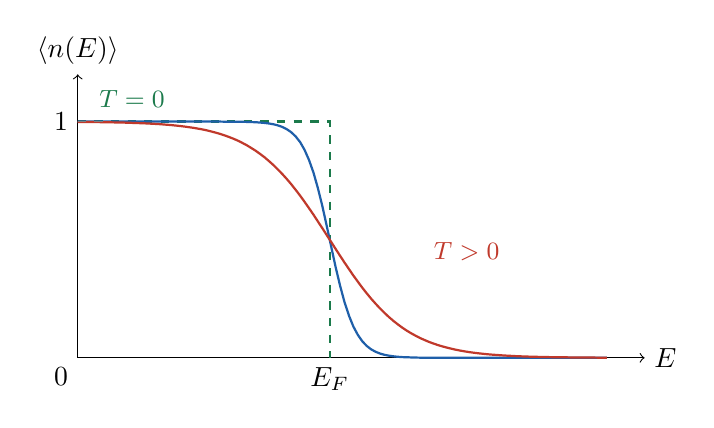
\begin{tikzpicture}
		\draw [->] (0,0) -- (7.2,0) node [right] {$E$};
		\draw [->] (0,0) -- (0,3.6) node [above] {$\avg{n(E)}$};
		\draw [thick, dashed, mgreen] plot coordinates {(0.000,3.000) (3.200,3.000) (3.200,0.000)};
		\draw [thick, mblue] plot coordinates {(0.000,3.000) (0.056,3.000) (0.113,3.000) (0.169,3.000) (0.226,3.000) (0.282,3.000) (0.339,3.000) (0.395,3.000) (0.452,3.000) (0.508,3.000) (0.565,3.000) (0.621,3.000) (0.678,3.000) (0.734,3.000) (0.791,3.000) (0.847,3.000) (0.904,3.000) (0.960,3.000) (1.016,3.000) (1.073,3.000) (1.129,3.000) (1.186,3.000) (1.242,3.000) (1.299,3.000) (1.355,3.000) (1.412,3.000) (1.468,3.000) (1.525,3.000) (1.581,3.000) (1.638,3.000) (1.694,3.000) (1.751,3.000) (1.807,3.000) (1.864,2.999) (1.920,2.999) (1.976,2.999) (2.033,2.998) (2.089,2.997) (2.146,2.996) (2.202,2.994) (2.259,2.992) (2.315,2.988) (2.372,2.983) (2.428,2.976) (2.485,2.966) (2.541,2.952) (2.598,2.932) (2.654,2.904) (2.711,2.865) (2.767,2.812) (2.824,2.740) (2.880,2.642) (2.936,2.515) (2.993,2.355) (3.049,2.158) (3.106,1.929) (3.162,1.676) (3.219,1.412) (3.275,1.153) (3.332,0.915) (3.388,0.707) (3.445,0.534) (3.501,0.396) (3.558,0.290) (3.614,0.210) (3.671,0.150) (3.727,0.107) (3.784,0.076) (3.840,0.054) (3.896,0.038) (3.953,0.027) (4.009,0.019) (4.066,0.013) (4.122,0.009) (4.179,0.007) (4.235,0.005) (4.292,0.003) (4.348,0.002) (4.405,0.002) (4.461,0.001) (4.518,0.001) (4.574,0.001) (4.631,0.000) (4.687,0.000) (4.744,0.000) (4.800,0.000) (4.856,0.000) (4.913,0.000) (4.969,0.000) (5.026,0.000) (5.082,0.000) (5.139,0.000) (5.195,0.000) (5.252,0.000) (5.308,0.000) (5.365,0.000) (5.421,0.000) (5.478,0.000) (5.534,0.000) (5.591,0.000) (5.647,0.000) (5.704,0.000) (5.760,0.000) (5.816,0.000) (5.873,0.000) (5.929,0.000) (5.986,0.000) (6.042,0.000) (6.099,0.000) (6.155,0.000) (6.212,0.000) (6.268,0.000) (6.325,0.000) (6.381,0.000) (6.438,0.000) (6.494,0.000) (6.551,0.000) (6.607,0.000) (6.664,0.000) (6.720,0.000)};
		\draw [thick, mred] plot coordinates {(0.000,2.996) (0.056,2.996) (0.113,2.995) (0.169,2.995) (0.226,2.994) (0.282,2.993) (0.339,2.992) (0.395,2.991) (0.452,2.990) (0.508,2.989) (0.565,2.988) (0.621,2.986) (0.678,2.984) (0.734,2.982) (0.791,2.980) (0.847,2.978) (0.904,2.975) (0.960,2.972) (1.016,2.969) (1.073,2.965) (1.129,2.960) (1.186,2.956) (1.242,2.950) (1.299,2.944) (1.355,2.937) (1.412,2.929) (1.468,2.921) (1.525,2.911) (1.581,2.901) (1.638,2.889) (1.694,2.875) (1.751,2.860) (1.807,2.844) (1.864,2.825) (1.920,2.805) (1.976,2.783) (2.033,2.758) (2.089,2.730) (2.146,2.700) (2.202,2.666) (2.259,2.630) (2.315,2.590) (2.372,2.547) (2.428,2.499) (2.485,2.448) (2.541,2.393) (2.598,2.334) (2.654,2.272) (2.711,2.205) (2.767,2.134) (2.824,2.060) (2.880,1.982) (2.936,1.902) (2.993,1.819) (3.049,1.733) (3.106,1.647) (3.162,1.559) (3.219,1.471) (3.275,1.383) (3.332,1.295) (3.388,1.210) (3.445,1.126) (3.501,1.044) (3.558,0.966) (3.614,0.890) (3.671,0.818) (3.727,0.750) (3.784,0.686) (3.840,0.626) (3.896,0.570) (3.953,0.517) (4.009,0.469) (4.066,0.424) (4.122,0.383) (4.179,0.345) (4.235,0.311) (4.292,0.280) (4.348,0.251) (4.405,0.226) (4.461,0.202) (4.518,0.181) (4.574,0.162) (4.631,0.145) (4.687,0.130) (4.744,0.116) (4.800,0.103) (4.856,0.092) (4.913,0.082) (4.969,0.073) (5.026,0.065) (5.082,0.058) (5.139,0.052) (5.195,0.046) (5.252,0.041) (5.308,0.037) (5.365,0.033) (5.421,0.029) (5.478,0.026) (5.534,0.023) (5.591,0.020) (5.647,0.018) (5.704,0.016) (5.760,0.014) (5.816,0.013) (5.873,0.011) (5.929,0.010) (5.986,0.009) (6.042,0.008) (6.099,0.007) (6.155,0.006) (6.212,0.006) (6.268,0.005) (6.325,0.004) (6.381,0.004) (6.438,0.004) (6.494,0.003) (6.551,0.003) (6.607,0.002) (6.664,0.002) (6.720,0.002)};
		\draw [dashed, gray] (0,3.000) -- (0.4,3.000);
		\node [left] at (0,3.000) {$1$};
		\node [below] at (3.200,0) {$E_F$};
		\node [mgreen, above right] at (0.15,3.05) {\small $T=0$};
		\node [mred, right] at (4.4,1.35) {\small $T>0$};
		\node [below left] at (0,0) {$0$};
	\end{tikzpicture}
\end{center}

This picture is the key to everything. Only the fermions within about $kT$ of the Fermi surface can be excited at all; those deep inside cannot move, because all the nearby states are occupied. So of the $N$ particles, only a fraction $\sim T/T_F$ participate in thermal physics, where $kT_F = E_F$ defines the \vocab{Fermi temperature}. Each of those carries $\sim kT$ of thermal energy, so
$$
E_{\mathrm{tot}} \approx \frac 35 NE_F + N\frac{T}{T_F}kT \implies C_V \sim Nk \frac{T}{T_F}.
$$
A more careful calculation, using the \vocab{Sommerfeld expansion} (which exploits the fact that $-\partial \avg n/\partial E$ is sharply peaked at $\mu$), gives the exact coefficient:
$$
C_V = \frac{\pi^2}{2}Nk\frac{T}{T_F} + O(T^3).
$$
The essential point is that $C_V \propto T$, linearly, and is suppressed by a factor $T/T_F$ relative to the classical value $\tfrac 32 Nk$.

\begin{example}[Electrons in metals]
	The conduction electrons in a metal form a Fermi gas of density $N/V \sim 10^{29}\,\mathrm{m}^{-3}$, giving $E_F$ of a few electronvolts and hence $T_F \sim 10^4$--$10^5\,\mathrm{K}$. Room temperature is therefore \emph{extremely} cold for the electrons: $T/T_F \sim 10^{-2}$, and the gas is highly degenerate.

	This resolves an old puzzle. In the nineteenth century it was known that metals conduct heat and electricity because they contain free electrons; but classically those electrons should contribute $\tfrac 32 Nk$ to the heat capacity, and no such contribution was observed. The answer is that the electronic heat capacity is suppressed by $T/T_F \sim 10^{-2}$, and is thus swamped by the phonons at ordinary temperatures. At very low temperature, though, the phonon contribution dies as $T^3$ while the electronic one dies only as $T$, so the electrons win. Indeed for a metal at low temperature
	$$
	C \approx \gamma T + \alpha T^3,
	$$
	and plotting $C/T$ against $T^2$ gives a straight line -- which is exactly what is measured.
\end{example}

\begin{example}[White dwarf stars]
	A star supports itself against gravity by thermal pressure, generated by nuclear fusion. When the fuel runs out, the star collapses -- and for a star of modest mass the collapse is halted by the degeneracy pressure of its electrons. The result is a \vocab{white dwarf}: an object of roughly the mass of the Sun compressed to the size of the Earth.

	We can estimate the equilibrium radius by balancing energies. The gravitational energy of a ball of mass $M$ and radius $R$ is $E_{\mathrm{grav}} \sim -GM^2/R$. The star contains $N \sim M/m_p$ nucleons and a comparable number of electrons, so the electron density is $n \sim N/R^3$ and the degeneracy energy is
	$$
	E_{\mathrm{deg}} \sim N E_F \sim N \frac{\hbar^2}{m_e}\left(\frac{N}{R^3}\right)^{2/3} = \frac{\hbar^2 N^{5/3}}{m_e R^2}.
	$$
	Minimising $E_{\mathrm{grav}} + E_{\mathrm{deg}}$ over $R$ gives
	$$
	R \sim \frac{\hbar^2}{G m_e m_p^{5/3} M^{1/3}},
	$$
	so, curiously, heavier white dwarfs are \emph{smaller}. Putting in the numbers for $M = M_\odot$ gives $R$ of a few thousand kilometres, which is right.

	The relation $R \propto M^{-1/3}$ cannot continue indefinitely. As $M$ increases, $R$ falls, the density rises, and eventually the electrons become relativistic. For an ultrarelativistic gas $E = \hbar c k$, and repeating the computation gives $E_{\mathrm{deg}} \sim \hbar c N^{4/3}/R$ -- which scales as $1/R$, exactly like the gravitational energy. The two therefore compete on equal terms, and if $M$ exceeds a critical value gravity wins and there is no equilibrium at all. This is the \vocab{Chandrasekhar limit}, about $1.4 M_\odot$; heavier remnants collapse to neutron stars or black holes.
\end{example}

\subsection{Pauli Paramagnetism}

As a final application, consider what happens when we put a Fermi gas in a magnetic field $B$. Each electron has a magnetic moment, so the energy of an electron of momentum $\vv k$ is
$$
E_\pm = \frac{\hbar^2 k^2}{2m} \pm \mu_B B,
$$
where $\mu_B = e\hbar/2m_e$ is the Bohr magneton and the sign depends on whether the spin is aligned or anti-aligned. Classically, one would expect the moments to align with the field, giving a susceptibility that diverges as $T \to 0$ (Curie's law $\chi \propto 1/T$). What actually happens is quite different.

The two spin species have shifted densities of states, $g_\pm(E) = \tfrac 12 g(E \mp \mu_B B)$. The magnetisation is
$$
M = \mu_B (N_- - N_+) = \mu_B\int_0^\infty \dd E\; \frac{g_-(E) - g_+(E)}{e^{\beta(E-\mu)}+1}.
$$
For small $B$ we expand $g(E \mp \mu_B B) \approx g(E) \mp \mu_B B\, g'(E)$, so
$$
M \approx \mu_B^2 B \int_0^\infty \dd E\; \frac{g'(E)}{e^{\beta(E-\mu)}+1} \approx \mu_B^2 B\, g(E_F)
$$
at low temperature, where the last step integrates by parts and uses the fact that $-\partial\avg n/\partial E$ is a sharp spike at $E_F$. So the susceptibility is
$$
\chi = \frac{\partial M}{\partial B} \approx \mu_B^2 g(E_F),
$$
which is a \emph{constant}, independent of temperature. This is \vocab{Pauli paramagnetism}, and the physical reason is by now familiar: only the electrons within $kT$ of the Fermi surface can flip their spins, since the others have nowhere to flip to.

%%END%%

\end{document}
